\documentclass[xcolor=table,svgnames,10pt,french]{beamer}

\usepackage{fontspec-luatex}
\usepackage{polyglossia}
\usepackage{listings}
\usepackage{multirow}
\usepackage{textcomp}
\usepackage{tikz}
\usepackage{hyperref}
\usepackage{hhline}
\usepackage{graphicx}
\usepackage{url}
\usepackage{amsmath,amssymb}
\usepackage{algorithm}
\usepackage{algpseudocode}
\usepackage{tabularx}
\usepackage{soul}
\usepackage[binary-units]{siunitx}
\usepackage[cache=false]{minted}
\usepackage{tcolorbox}

\usetikzlibrary{arrows,automata,backgrounds,shapes,snakes,patterns,decorations, shapes.arrows, positioning}

\setmainlanguage{french}

\usetheme{metropolis}

\definecolor{maDarkBrown}{HTML}{604c38}
\definecolor{maDarkTeal}{HTML}{23373b}
\definecolor{maLightBrown}{HTML}{EB811B}
\definecolor{maLightGreen}{HTML}{14B03D}

\newenvironment<>{remarque}[1][\undefined]{%
  \begin{actionenv}#2%
    \ifx#1\undefined%
    \def\insertblocktitle{Remarque}%
    \else%
    \def\insertblocktitle{Remarque ({\em#1})}%
    \fi%
    \par%
    \mode<presentation>{%
      \setbeamercolor{block title}{fg=black,bg=maLightGreen!50}
      \setbeamercolor{block body}{fg=black,bg=maLightGreen!20}
    }%
    \usebeamertemplate{block begin}\em}
  {\par\usebeamertemplate{block end}\end{actionenv}}



\newcommand{\demo}[0]{%
  \hfill\begin{tcolorbox}[hbox,colback=maLightGreen!50,colframe=maLightGreen,halign=flushleft]\bf → Démo\end{tcolorbox}}

\hypersetup{
  colorlinks=true
}

\title[R2.04]{Ressource R2.04 \\ Communication et fonctionnement bas niveau}
\subtitle{Cours n°1 \\Organisation d'un ordinateur \\Exécution d'un programme}
\author[Loïg Jezequel, Jean-Luc Béchennec, Sébastien Faucou, Olivier Boutin]{}
\date{version du \today}

\AtBeginSection[]
{
  \frame{
    \frametitle{Plan du cours}
    \tableofcontents[currentsection, sectionstyle=show/shaded,subsectionstyle=show/show/hide]
  }
}

\AtBeginSubsection[]
{
  \frame{
    \frametitle{Plan du cours}
    \tableofcontents[currentsection, currentsubsection, subsectionstyle=show/shaded/hide]
  }
}


\AtBeginSubsubsection[]
{
  \frame{
    \frametitle{Plan du cours}
    \tableofcontents[currentsection, currentsubsection, subsubsectionstyle=show/shaded/hide/hide]
  }
}

\begin{document}

\frame{
  \maketitle
}

\begin{frame}
    \frametitle{D'après le programme natiional du BUT INFO}

  \begin{block}{Descriptif}
    \small
    L’objectif de cette ressource est de comprendre \alert<2>{le fonctionnement des couches systèmes} et réseaux \alert<2>{bas niveau}.
    Cette ressource permet de découvrir les multiples technologies et fonctions mises en œuvre dans un réseau informatique et de comprendre les rôles et structures des mécanismes bas niveau mis en \oe{}uvre pour leur fonctionnement.
  \end{block}

  \begin{block}{Savoirs de référence étudiés}
    \small
    \begin{itemize}
      \item \alert<2>{Étude d’un système à microprocesseur} ou microcontrôleur avec ses composants (mémoires, interfaces, périphériques...)
      \item \alert<2>{Langages de programmation de bas niveau et mécanismes de bas niveau d’un système informatique}
      \item Étude d’architectures de réseaux et notion de pile protocolaire
      \item Technologie des réseaux locaux : Ethernet, wifi, TCP/IP, routage, commutation, adressage, transport
    \end{itemize}
  \end{block}

  \begin{block}{Mots clés}
    \small
    Protocoles – \alert<2>{Pointeurs} – Interruptions – \alert<2>{Langage bas niveau}
  \end{block}


\end{frame}

\section{Exécution d'un programme}

\subsection{Du code de haut niveau à l'exécutable}

\begin{frame}[fragile]
  \frametitle{Exemple}

\begin{minted}{go}
package main

import "fmt"

func main() {
  var hello = "Hello, BUT"
  var helloAsRuneArray = []rune(hello)
  for i := 0; i < len(helloAsRuneArray); i++ {
    fmt.Print(string(helloAsRuneArray[i]), ".")
  }
  fmt.Println()
}
\end{minted}

  On souhaite exécuter ce programme. Quelles étapes doit-on suivre ?

\end{frame}

\begin{frame}

    La commande \texttt{go build} enchaîne plusieurs étapes :

    \begin{enumerate}
        \item Compilation (langage de haut niveau → code objet)
            \begin{enumerate}
                \item Analyse lexicale
                \item Analyse syntaxique
                \item Analyse sémantique
                \item Traduction en code intermédiaire
                \item Optimisations
                \item Génération du code objet et assemblage
            \end{enumerate}
        \item Édition des liens (codes objets → exécutable)
            \begin{enumerate}
                \item Résolution des liens
                \item Optimisations 
                \item Génération du code exécutable
            \end{enumerate}
    \end{enumerate}

\end{frame}

\begin{frame}
   
    Quelques commandes pour voir ce qui se passe :

    \begin{exampleblock}{Afficher toutes les commandes enchaînées}
        \texttt{go build -x -work}
    \end{exampleblock}

    \begin{exampleblock}{Obtenir le code avant assemblage}
        \texttt{go build -gcflags="-S" 2> main.S}
    \end{exampleblock}
   
    \begin{exampleblock}{Désassembler le code exécutable}
        \texttt{objdump -d hello > hello.d}
    \end{exampleblock}

    → Dans le code désassemblé, en plus du code correspondant à la traduction du code source, on trouve :
    \begin{itemize}
        \item du code spécifique au système d'exploitation,
        \item du code venant du \textit{runtime} go.
    \end{itemize}
\end{frame}

\begin{frame} 
    \frametitle{Langage machine (1)}

    Un exécutable contient un programme exprimé en \emph{langage machine}.

    C'est un langage de bas niveau, très proche du matériel.

    Un programme en langage machine peut être exprimé de deux façons :
    \begin{itemize}
        \item \alert{en binaire} -- représentation utilisée en mémoire
        \item \alert{en texte} -- représentation utilisée pour écrire / déboguer le code machine
    \end{itemize}

    \begin{center}
    \begin{tikzpicture}
        \node (text) {texte};
        \node (bin) [right=3cm of text] {binaire};
        \draw[->] (text) to [bend right] node[below, midway] {\small assemblage} (bin);
        \draw[->] (bin) to [bend right] node[above, midway] {\small désassemblage} (text);
    \end{tikzpicture}
    \end{center}

\end{frame}

\begin{frame}
    \frametitle{Langage machine (2)}

    Le langage machine est très différents des langages de haut niveau :

    \begin{itemize}
        \item Il y a beaucoup d'instructions, construite sur le même schéma.
            \begin{itemize}
                \item un \alert{opcode} : identifie l'opération
                \item des \alert{opérandes sources et cibles} : registre, adresse mémoire, ou constante entière
            \end{itemize}
        \item Le nombre, les noms, et la taille des variables sont connues à l'avance :
            \begin{itemize}
                \item les \alert{registres} ;
                \item la \alert{mémoire de travail} = un tableau d'octets, qui contient le code et les variables.
            \end{itemize}
        \item Il n'y a pas de type, ou plutôt il n'y a qu'un type : les entiers de taille fixe.
    \end{itemize}

\end{frame}

\begin{frame}{Langage machine (3)}

    Les opérations relèvent très majoritairement des catégories suivantes :

    \medskip

    \begin{itemize}
        \item \alert{accès à  la mémoire de travail} : copie de données entre la mémoire de travail et les registres ;
        \item \alert{instruction arithmétique ou logique} : opération sur des données présentes dans les registres, des constantes ;
        \item \alert{branchement (ou saut)} : détournement du flot de contrôle normal, utilisés pour les appels de procédures, les conditionnels, les boucles.
    \end{itemize}

    \medskip

    Il existe d'autres opérations permettant d'interagir avec les périphériques ou de contrôler l'état de la machine.
\end{frame}

\begin{frame}
    \frametitle{Langage machine (4)}

    Le langage machine est également appelé \alert{jeu d'instruction} (\emph{instruction set architecture} en anglais, abbr. ISA).

    On distingue habituellement deux catégories d'ISA :

    \begin{block}{Complex Instruction Set Computer (CISC)}
        Beaucoup d'opérations, dont certaines complexes, pouvant relever de plusieurs catégories.
        Code compact, parfois difficile à optimiser.
        Implémentation complexe mais permet d'optimiser fortement certaines instructions.
    \end{block}

    \begin{block}{Reduced Instruction Set Computer (RISC)}
        Peu d'opérations, chacune relevant d'une unique catégorie.
        Code plus verbeux, mais plus simple à optimiser.
        Implémentation simple et souvent efficace sur le plan énergétique.
    \end{block}
\end{frame}

\begin{frame}[fragile]
    \frametitle{Langage machine (5)}

    \begin{columns}[T]
        \begin{column}{.5\textwidth}
            \small
\begin{minted}{go}
func add(a, b int) (res int) {
    res = a + b
    return
}
\end{minted}
        \end{column}
        \begin{column}{.5\textwidth}
            \small
\begin{minted}{GAS}
push   %rbp
mov    %rsp,%rbp
sub    $0x8,%rsp
mov    %rax,0x18(%rsp)
mov    %rbx,0x20(%rsp)
movq   $0x0,(%rsp)
add    %rbx,%rax
mov    %rax,(%rsp)
add    $0x8,%rsp
pop    %rbp
ret
\end{minted}
        \end{column}
    \end{columns}

    \medskip

    Remarque : quand on désactive les optimisations, le code produit par le compilateur comporte des instructions « inutiles ».
\end{frame}


\begin{frame}[fragile]
    \frametitle{Langage machine (6)}

    \begin{columns}[T]
        \begin{column}{.5\textwidth}
            \small
\begin{minted}{go}
func add(a, b int) (res int) {
    res = a + b
    return
}
\end{minted}
        \end{column}
        \begin{column}{.5\textwidth}
            \small
\begin{minted}{GAS}
add    %rbx,%rax
ret
\end{minted}
        \end{column}
    \end{columns}

    \medskip

    Remarque : dans le code optimisé, la fonction n'est même pas appelée (le compilateur pré-calcule le résultat et le fait directement afficher). 
\end{frame}

\subsection{L'exécution}

\begin{frame}

    Pour « lancer le programme », le système d'exploitation doit réaliser plusieurs opérations, dont :

    \begin{itemize}
        \item créér un nouveau \alert{processus} et lui associer un \alert{espace d'adressage virtuel} ;
        \item charger dans cet espace d'adressage le code et les données du programme (copie disque → mémoire de travail) ;
        \item initialiser les autres zones de l'espace d'adressage (en particulier : \alert{pile} et \alert{tas}) ;
        \item initaliser les \alert{descripteurs de ressources} associés à ce processus (entre autres : fichiers ouverts, dont entrée standard et sortie standard) ;
        \item charger dans le \alert{pointeur d'instruction} l'adresse du point d'entrée du programme.
    \end{itemize}

\end{frame}

\frame{
  \frametitle{Schéma de principe d'un ordinateur}

  \centering
  \scalebox{0.7}{%\documentclass{report}
%\usepackage{fullpage}
%\usepackage{tikz}
%\usepackage[utf8]{inputenc}
%\usepackage[OT1]{fontenc}

%\begin{document}

\begin{tikzpicture}

\newcommand{\myarrowright}[3]{% x depart, y depart, longueur
\draw[black!25,fill=black!25] (#1,#2+0.25) -- (#1+#3-0.5,#2+0.25) -- (#1+#3-0.5,#2+0.5) -- (#1+#3,#2) -- (#1+#3-0.5,#2-0.5) -- (#1+#3-0.5,#2-0.25) -- (#1,#2-0.25) -- (#1,#2+0.25);
}
\newcommand{\myarrowleft}[3]{% x depart, y depart, longueur
\draw[black!25,fill=black!25] (#1,#2+0.25) -- (#1-#3+0.5,#2+0.25) -- (#1-#3+0.5,#2+0.5) -- (#1-#3,#2) -- (#1-#3+0.5,#2-0.5) -- (#1-#3+0.5,#2-0.25) -- (#1,#2-0.25) -- (#1,#2+0.25);
}
\newcommand{\myarrowup}[3]{% x depart, y depart, longueur
\draw[black!25,fill=black!25] (#1+0.25,#2) -- (#1+0.25,#2+#3-0.5) -- (#1+0.5,#2+#3-0.5) -- (#1,#2+#3) -- (#1-0.5,#2+#3-0.5) -- (#1-0.25,#2+#3-0.5) -- (#1-0.25,#2) -- (#1+0.25,#2);
}
\newcommand{\myarrowdown}[3]{% x depart, y depart, longueur
\draw[black!25,fill=black!25] (#1+0.25,#2) -- (#1+0.25,#2-#3+0.5) -- (#1+0.5,#2-#3+0.5) -- (#1,#2-#3) -- (#1-0.5,#2-#3+0.5) -- (#1-0.25,#2-#3+0.5) -- (#1-0.25,#2) -- (#1+0.25,#2);
}


%% \foreach \i in {0,...,15} {
%%   \foreach \j in {-20,...,0} {
%%     \node[black!25] at (\i,\j) {\i,\j};
%%   }
%% }

%cpu
\draw (0,0) rectangle (7,-6);
\node at (8.25,-0.25) {\Large Processeur};
%bus registers->ALU
\myarrowright{3.75}{-1.5}{1.25}
%bus ALU->registers
\myarrowleft{5}{-3}{1.25}
%bus CPU->i/o bridge
\myarrowright{6}{-5.25}{2}
%bus i/o bridge->CPU
\myarrowleft{7}{-5.25}{2}
%bus i/o brige->memory
\myarrowright{11}{-5.25}{2.5}
%bus memory->i/o bridge
\myarrowleft{11}{-5.25}{1}
%i/o bus->i/o bridge
\myarrowup{9}{-7}{1.25}
%bus interface->registers
\myarrowup{3}{-4}{0.5}
%registers->bus interface
\myarrowdown{3}{-4}{0.75}
%i/o bus->usb controller
\myarrowdown{2}{-7.25}{1.5}
%i/o bus->graphics adapter
\myarrowdown{6}{-7.25}{1.5}
%i/o bus->disk controller
\myarrowdown{10}{-7.25}{1.5}
%pc
\draw (0.5,-1.75) rectangle (2,-2.25);
\node at (1.25,-2) {\Large PC};
%other registers
\draw (2.25,-1) rectangle (3.75,-3.5);
\draw (2.25,-1.5) -- (3.75,-1.5);
\draw (2.25,-2) -- (3.75,-2);
\draw (2.25,-2.5) -- (3.75,-2.5);
\draw (2.25,-3) -- (3.75,-3);
\node at (2,-0.5) {\Large Registres};
%alu
\draw (5,-0.5) rectangle (6.5,-4);
\node at (5.75,-2.25) {\Large UAL};
%bus interface
\draw (0.5,-4.75) rectangle (5,-5.75);
\node at (2.75,-5.25) {\Large Interface};
%i/o bridge
\draw (8,-4.75) rectangle (10,-5.75);
\node at (9,-5.25) {\large Pont e/s};
%memory
\draw (13.5,-4) rectangle (15.5,-6);
\node at (14.5,-5) {\Large Mémoire};
%i/o bus
\myarrowleft{8}{-7.25}{8}
\myarrowright{8}{-7.25}{7.5}
%usb controller
\draw (1,-8.75) rectangle (3,-9.75);
\node at (2,-9) {\large Contrôleur};
\node at (2,-9.5) {\large USB};
\draw[-latex] (1.25,-10.5) -- (1.25,-9.75);
\node at (1.25,-10.75) {\Large Clavier~~~};
\draw[-latex] (2.75,-10.5) -- (2.75,-9.75);
\node at (2.75,-10.75) {\Large ~~~Souris};
%graphics adapter
\draw (4.95,-8.75) rectangle (7.05,-9.75);
\node at (6,-9) {\large Adaptateur};
\node at (6,-9.5) {\large graphique};
\draw[-latex] (6,-9.75) -- (6,-10.5);
\node at (6,-10.75) {\Large Écran};
%disk controller
\draw (9,-8.75) rectangle (11,-9.75);
\node at (10,-9) {\large Contrôleur};
\node at (10,-9.5) {\large stockage};
\draw[-latex] (11,-9.25) -- (12.5,-9.25);
\draw[-latex] (12.5,-9.25) -- (11,-9.25);
%disk
\draw (12.5,-8.5) rectangle (14.5,-10.5);
\node at (13.5,-9.5) {\Large Stockage};
%bus names
\node at (7.5,-7.25) {\large Bus e/s};
\node at (11.75,-5.25) {\large Bus mémoire};
\node at (6.5,-5.25) {\large Bus système};


\end{tikzpicture}

%\end{document}
}

}

\frame{

  \centering
  \scalebox{0.7}{%% \documentclass{report}
%% \usepackage{fullpage}
%% \usepackage{tikz}
%% \usepackage[utf8]{inputenc}
%% \usepackage[OT1]{fontenc}

%% \begin{document}

\begin{tikzpicture}

\newcommand{\myarrowright}[3]{% x depart, y depart, longueur
\draw[black!25,fill=black!25] (#1,#2+0.25) -- (#1+#3-0.5,#2+0.25) -- (#1+#3-0.5,#2+0.5) -- (#1+#3,#2) -- (#1+#3-0.5,#2-0.5) -- (#1+#3-0.5,#2-0.25) -- (#1,#2-0.25) -- (#1,#2+0.25);
}
\newcommand{\myarrowleft}[3]{% x depart, y depart, longueur
\draw[black!25,fill=black!25] (#1,#2+0.25) -- (#1-#3+0.5,#2+0.25) -- (#1-#3+0.5,#2+0.5) -- (#1-#3,#2) -- (#1-#3+0.5,#2-0.5) -- (#1-#3+0.5,#2-0.25) -- (#1,#2-0.25) -- (#1,#2+0.25);
}
\newcommand{\myarrowup}[3]{% x depart, y depart, longueur
\draw[black!25,fill=black!25] (#1+0.25,#2) -- (#1+0.25,#2+#3-0.5) -- (#1+0.5,#2+#3-0.5) -- (#1,#2+#3) -- (#1-0.5,#2+#3-0.5) -- (#1-0.25,#2+#3-0.5) -- (#1-0.25,#2) -- (#1+0.25,#2);
}
\newcommand{\myarrowdown}[3]{% x depart, y depart, longueur
\draw[black!25,fill=black!25] (#1+0.25,#2) -- (#1+0.25,#2-#3+0.5) -- (#1+0.5,#2-#3+0.5) -- (#1,#2-#3) -- (#1-0.5,#2-#3+0.5) -- (#1-0.25,#2-#3+0.5) -- (#1-0.25,#2) -- (#1+0.25,#2);
}


%% \foreach \i in {0,...,15} {
%%   \foreach \j in {-20,...,0} {
%%     \node[black!25] at (\i,\j) {\i,\j};
%%   }
%% }

%cpu
\draw (0,0) rectangle (7,-6);
\node at (8.25,-0.25) {\Large Processeur};
%bus registers->ALU
\myarrowright{3.75}{-1.5}{1.25}
%bus ALU->registers
\myarrowleft{5}{-3}{1.25}
%bus CPU->i/o bridge
\myarrowright{6}{-5.25}{2}
%bus i/o bridge->CPU
\myarrowleft{7}{-5.25}{2}
%bus i/o brige->memory
\myarrowright{11}{-5.25}{2.5}
%bus memory->i/o bridge
\myarrowleft{11}{-5.25}{1}
%i/o bus->i/o bridge
\myarrowup{9}{-7}{1.25}
%bus interface->registers
\myarrowup{3}{-4}{0.5}
%registers->bus interface
\myarrowdown{3}{-4}{0.75}
%i/o bus->usb controller
\myarrowdown{2}{-7.25}{1.5}
%i/o bus->graphics adapter
\myarrowdown{6}{-7.25}{1.5}
%i/o bus->disk controller
\myarrowdown{10}{-7.25}{1.5}
%pc
\draw (0.5,-1.75) rectangle (2,-2.25);
\node at (1.25,-2) {\Large PC};
%other registers
\draw (2.25,-1) rectangle (3.75,-3.5);
\draw (2.25,-1.5) -- (3.75,-1.5);
\draw (2.25,-2) -- (3.75,-2);
\draw (2.25,-2.5) -- (3.75,-2.5);
\draw (2.25,-3) -- (3.75,-3);
\node at (2,-0.5) {\Large Registres};
%alu
\draw (5,-0.5) rectangle (6.5,-4);
\node at (5.75,-2.25) {\Large UAL};
%bus interface
\draw (0.5,-4.75) rectangle (5,-5.75);
\node at (2.75,-5.25) {\Large Interface};
%i/o bridge
\draw (8,-4.75) rectangle (10,-5.75);
\node at (9,-5.25) {\large Pont e/s};
%memory
\draw (13.5,-4) rectangle (15.5,-6);
\node at (14.5,-5) {\Large Mémoire};
%i/o bus
\myarrowleft{8}{-7.25}{8}
\myarrowright{8}{-7.25}{7.5}
%usb controller
\draw (1,-8.75) rectangle (3,-9.75);
\node at (2,-9) {\large Contrôleur};
\node at (2,-9.5) {\large USB};
\draw[-latex] (1.25,-10.5) -- (1.25,-9.75);
\node at (1.25,-10.75) {\Large Clavier~~~};
\draw[-latex] (2.75,-10.5) -- (2.75,-9.75);
\node at (2.75,-10.75) {\Large ~~~Souris};
%graphics adapter
\draw (4.95,-8.75) rectangle (7.05,-9.75);
\node at (6,-9) {\large Adaptateur};
\node at (6,-9.5) {\large graphique};
\draw[-latex] (6,-9.75) -- (6,-10.5);
\node at (6,-10.75) {\Large Écran};
%disk controller
\draw (9,-8.75) rectangle (11,-9.75);
\node at (10,-9) {\large Contrôleur};
\node at (10,-9.5) {\large disque};
\draw[-latex] (11,-9.25) -- (12.5,-9.25);
\draw[-latex] (12.5,-9.25) -- (11,-9.25);
%disk
\draw (12.5,-8.5) rectangle (14.5,-10.5);
\node at (13.5,-9.5) {\Large Stockage};
%bus names
\node at (7.5,-7.25) {\large Bus e/s};
\node at (11.75,-5.25) {\large Bus mémoire};
\node at (6.5,-5.25) {\large Bus système};


\draw[red,very thick,-latex] (12.75,-9) -- (10,-9) -- (10,-7.25) -- (9,-7.25) -- (9,-5.25) -- (13.6,-5.25);
\node[red] at (13.3,-9) {\large \tt hello};

\end{tikzpicture}

%\end{document}
}

}

\frame{
  \centering
  \scalebox{0.7}{%% \documentclass{report}
%% \usepackage{fullpage}
%% \usepackage{tikz}
%% \usepackage[utf8]{inputenc}
%% \usepackage[OT1]{fontenc}

%% \begin{document}

\begin{tikzpicture}

\newcommand{\myarrowright}[3]{% x depart, y depart, longueur
\draw[black!25,fill=black!25] (#1,#2+0.25) -- (#1+#3-0.5,#2+0.25) -- (#1+#3-0.5,#2+0.5) -- (#1+#3,#2) -- (#1+#3-0.5,#2-0.5) -- (#1+#3-0.5,#2-0.25) -- (#1,#2-0.25) -- (#1,#2+0.25);
}
\newcommand{\myarrowleft}[3]{% x depart, y depart, longueur
\draw[black!25,fill=black!25] (#1,#2+0.25) -- (#1-#3+0.5,#2+0.25) -- (#1-#3+0.5,#2+0.5) -- (#1-#3,#2) -- (#1-#3+0.5,#2-0.5) -- (#1-#3+0.5,#2-0.25) -- (#1,#2-0.25) -- (#1,#2+0.25);
}
\newcommand{\myarrowup}[3]{% x depart, y depart, longueur
\draw[black!25,fill=black!25] (#1+0.25,#2) -- (#1+0.25,#2+#3-0.5) -- (#1+0.5,#2+#3-0.5) -- (#1,#2+#3) -- (#1-0.5,#2+#3-0.5) -- (#1-0.25,#2+#3-0.5) -- (#1-0.25,#2) -- (#1+0.25,#2);
}
\newcommand{\myarrowdown}[3]{% x depart, y depart, longueur
\draw[black!25,fill=black!25] (#1+0.25,#2) -- (#1+0.25,#2-#3+0.5) -- (#1+0.5,#2-#3+0.5) -- (#1,#2-#3) -- (#1-0.5,#2-#3+0.5) -- (#1-0.25,#2-#3+0.5) -- (#1-0.25,#2) -- (#1+0.25,#2);
}


%% \foreach \i in {0,...,15} {
%%   \foreach \j in {-20,...,0} {
%%     \node[black!25] at (\i,\j) {\i,\j};
%%   }
%% }

%cpu
\draw (0,0) rectangle (7,-6);
\node at (8.25,-0.25) {\Large Processeur};
%bus registers->ALU
\myarrowright{3.75}{-1.5}{1.25}
%bus ALU->registers
\myarrowleft{5}{-3}{1.25}
%bus CPU->i/o bridge
\myarrowright{6}{-5.25}{2}
%bus i/o bridge->CPU
\myarrowleft{7}{-5.25}{2}
%bus i/o brige->memory
\myarrowright{11}{-5.25}{2.5}
%bus memory->i/o bridge
\myarrowleft{11}{-5.25}{1}
%i/o bus->i/o bridge
\myarrowup{9}{-7}{1.25}
%bus interface->registers
\myarrowup{3}{-4}{0.5}
%registers->bus interface
\myarrowdown{3}{-4}{0.75}
%i/o bus->usb controller
\myarrowdown{2}{-7.25}{1.5}
%i/o bus->graphics adapter
\myarrowdown{6}{-7.25}{1.5}
%i/o bus->disk controller
\myarrowdown{10}{-7.25}{1.5}
%pc
\draw (0.5,-1.75) rectangle (2,-2.25);
\node at (1.25,-2) {\Large PC};
%other registers
\draw (2.25,-1) rectangle (3.75,-3.5);
\draw (2.25,-1.5) -- (3.75,-1.5);
\draw (2.25,-2) -- (3.75,-2);
\draw (2.25,-2.5) -- (3.75,-2.5);
\draw (2.25,-3) -- (3.75,-3);
\node at (2,-0.5) {\Large Registres};
%alu
\draw (5,-0.5) rectangle (6.5,-4);
\node at (5.75,-2.25) {\Large UAL};
%bus interface
\draw (0.5,-4.75) rectangle (5,-5.75);
\node at (2.75,-5.25) {\Large Interface};
%i/o bridge
\draw (8,-4.75) rectangle (10,-5.75);
\node at (9,-5.25) {\large Pont e/s};
%memory
\draw (13.5,-4) rectangle (15.5,-6);
\node at (14.5,-5) {\Large Mémoire};
%i/o bus
\myarrowleft{8}{-7.25}{8}
\myarrowright{8}{-7.25}{7.5}
%usb controller
\draw (1,-8.75) rectangle (3,-9.75);
\node at (2,-9) {\large Contrôleur};
\node at (2,-9.5) {\large USB};
\draw[-latex] (1.25,-10.5) -- (1.25,-9.75);
\node at (1.25,-10.75) {\Large Clavier~~~};
\draw[-latex] (2.75,-10.5) -- (2.75,-9.75);
\node at (2.75,-10.75) {\Large ~~~Souris};
%graphics adapter
\draw (4.95,-8.75) rectangle (7.05,-9.75);
\node at (6,-9) {\large Adaptateur};
\node at (6,-9.5) {\large graphique};
\draw[-latex] (6,-9.75) -- (6,-10.5);
\node at (6,-10.75) {\Large Écran};
%disk controller
\draw (9,-8.75) rectangle (11,-9.75);
\node at (10,-9) {\large Contrôleur};
\node at (10,-9.5) {\large Stockage};
\draw[-latex] (11,-9.25) -- (12.5,-9.25);
\draw[-latex] (12.5,-9.25) -- (11,-9.25);
%disk
\draw (12.5,-8.5) rectangle (14.5,-10.5);
\node at (13.5,-9.5) {\Large Disque};
%bus names
\node at (7.5,-7.25) {\large Bus e/s};
\node at (11.75,-5.25) {\large Bus mémoire};
\node at (6.5,-5.25) {\large Bus système};


\draw[red,very thick] (3,-3) -- (5.75,-3) -- (5.75,-1.5) -- (3,-1.5) -- (3,-5.25) -- (13.6,-5.25);
\node[red] at (14.5,-5.5) {\large \tt hello};

\end{tikzpicture}

%\end{document}
}
}

\subsubsection{Zoom sur l'unité centrale}

\begin{frame}{Microarchitecture MIPS}

\begin{center}
    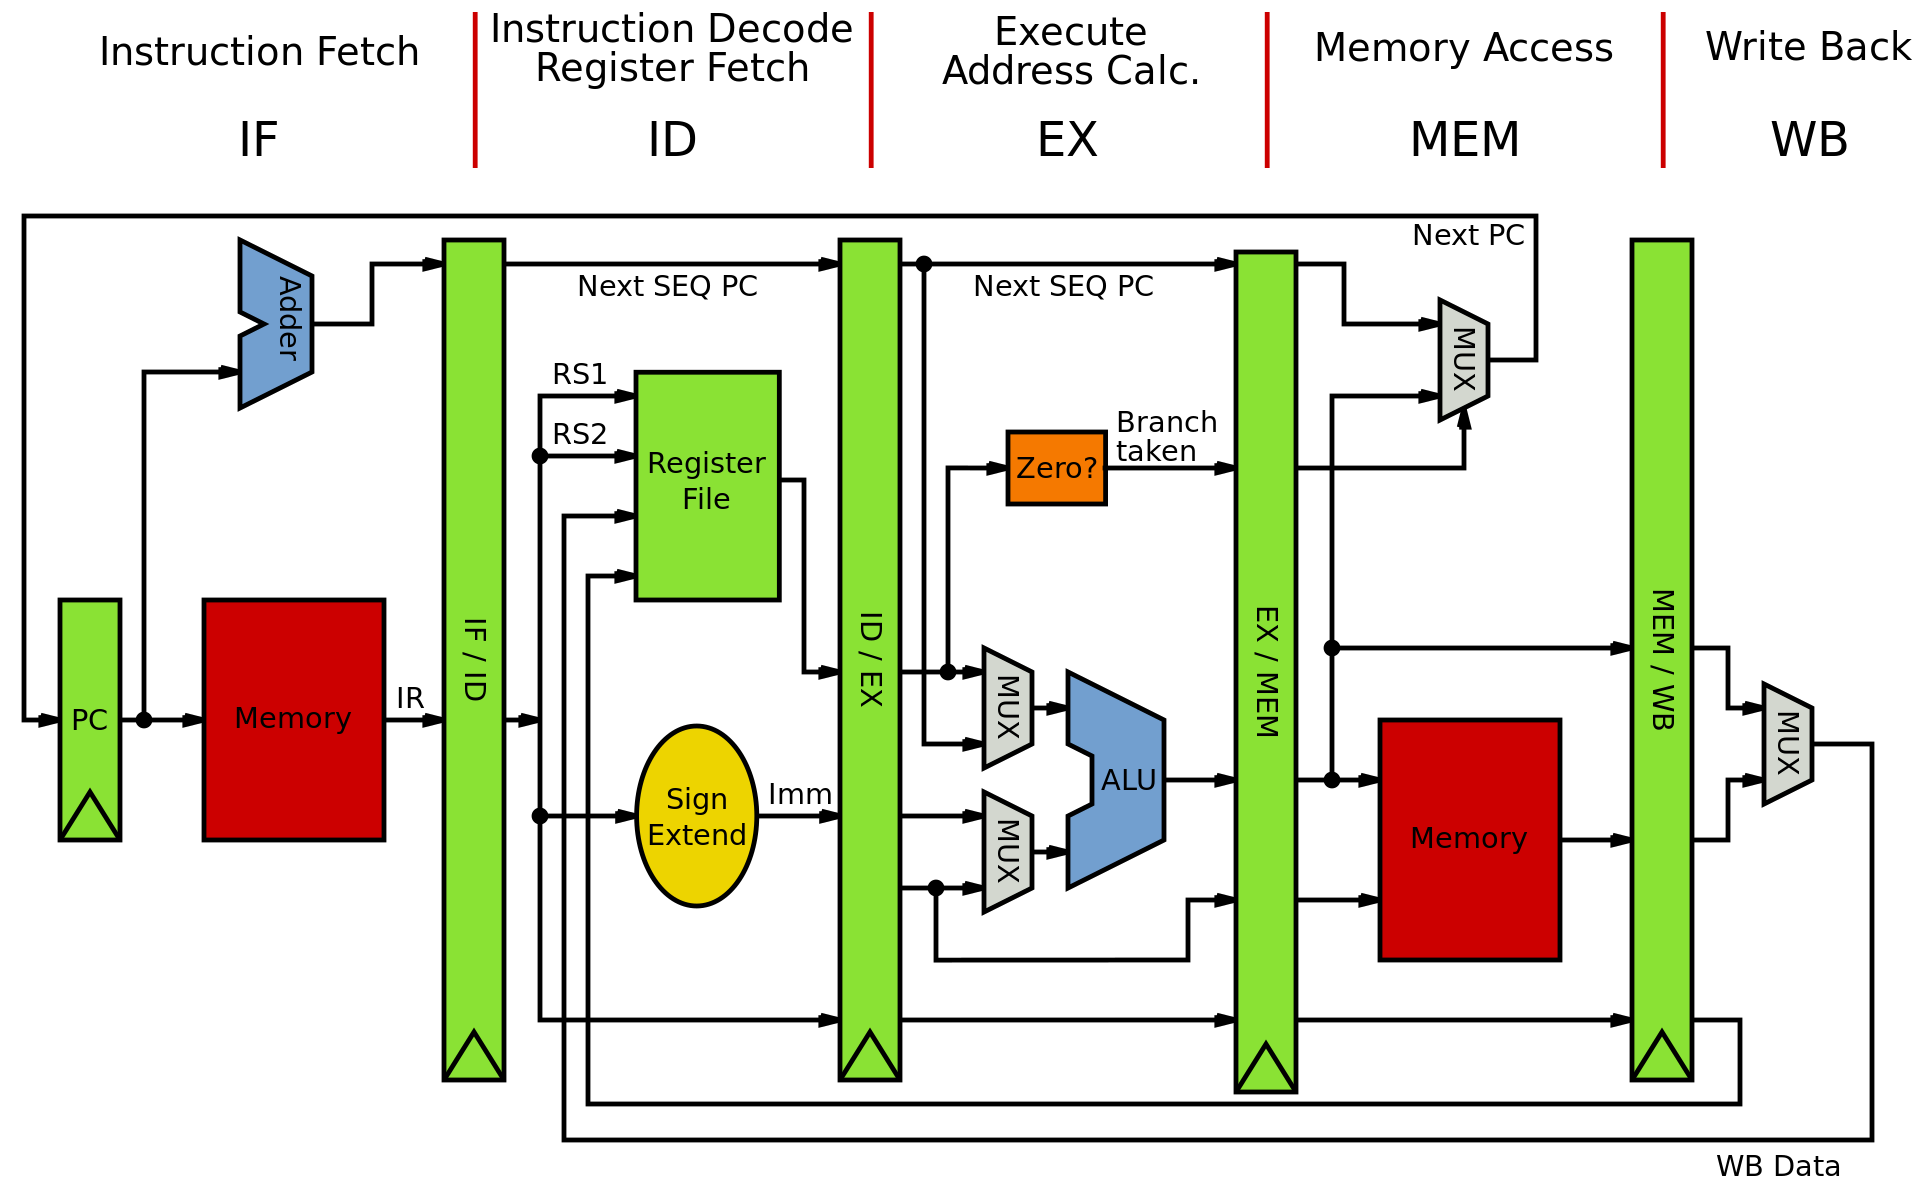
\includegraphics[width=.9\textwidth]{figures/MIPS_Architecture_(Pipelined).svg}
\end{center}
    Schéma de principe d'un processeur simple.
\end{frame}


\begin{frame}{Microarchitecture CVA6}

\begin{center}
    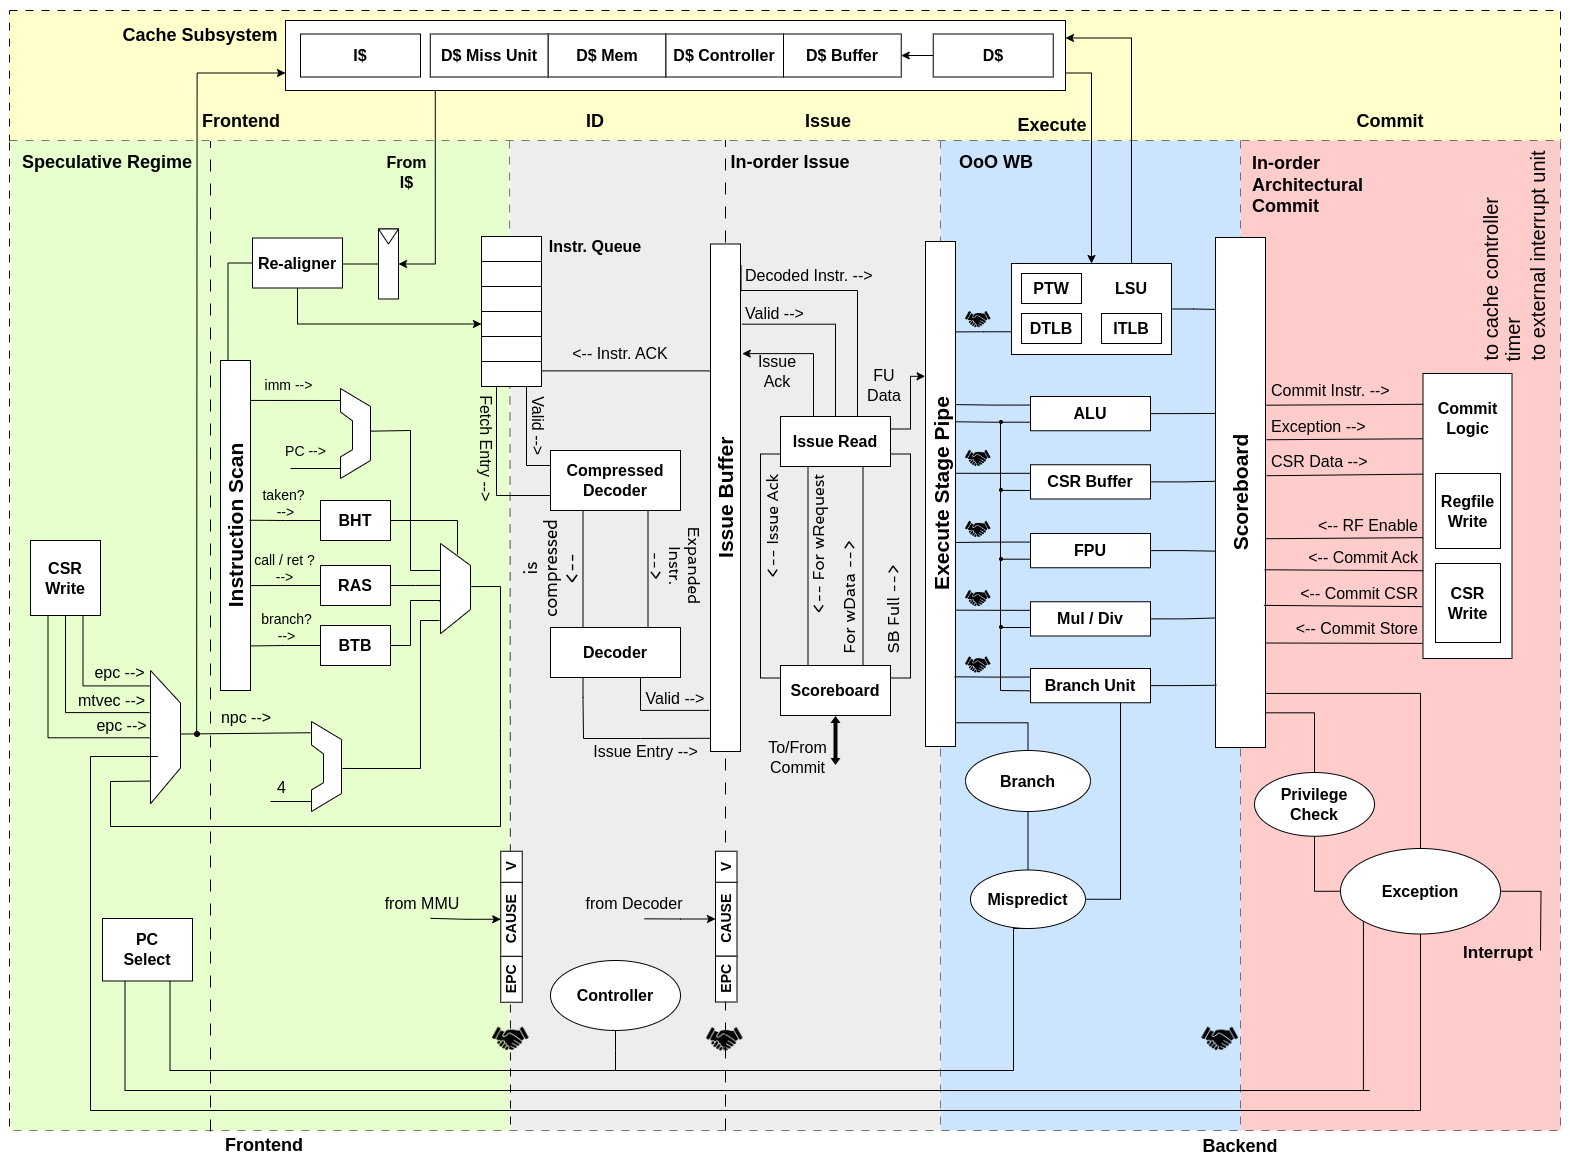
\includegraphics[width=.85\textwidth]{figures/ariane_overview.drawio.png}
\end{center}
    Schéma de principe d'un processeur un peu plus complexe intégrant des mécanismes de spéculation.
\end{frame}


\begin{frame}{Les registres}

    Fichier de registre : mémoire très petite mais accès quasi-immédiat (dans le processeur).
    Elle contient :
    \begin{itemize}
        \item l'état du processeur ;
        \item l'état du processus ;
        \item les valeurs en cours d'utilisation par le programme.
    \end{itemize}

    \medskip

    Taille d'un registre = taille d'une adresse mémoire (dépend de l'architecture, 32 ou 64 bits pour les architectures modernes).

    \medskip

    Chaque registre porte un nom utilisé pour le désigner comme opérande.

\end{frame}

\begin{frame}
    \frametitle{Les registres (2)}

    L'ISA spécifie un jeu de registre accessibles par les programmes 
    \begin{itemize}
        \item soit comme opérande explicite ;
        \item soit comme opérande de sortie implicite.
    \end{itemize}

    \medskip

    La microarchitecture contient souvent plus de registres :
    \begin{itemize}
        \item registres internes au pipeline ;
        \item ou étage d'allocation des registres ISA aux registres physiques.
    \end{itemize}

\end{frame}

\subsubsection{Zoom sur l'espace d'adressage virtuel}

\begin{frame}{Espace d'adressage virtuel}

        \begin{itemize}
            \item abstraction de la \alert{hiérarchie mémoire du système} ;
            \item au début : contient le code, les globales initialisées, les constantes, les paramètres, l'environnement ;
            \item vue du programme : un tableau de \alert{mots}
                \begin{itemize}
                    \item taille d'un mot : dépend de l'architecture → typiquement 4 ou 8 octets.
                    \item taille du tableau : dépend de l'architecture → typiquement $2^{32}$ ou $2^{64}$ octets.
                \end{itemize}
            \item organisation en \alert{sections} par le compilateur : pile, tas, programme, données.
        \end{itemize}
    
\end{frame}

\begin{frame}{Les sections}
    
    \begin{block}{La pile (\texttt{stack})}
        Utilisée pour gérer les appels de procédure :
        \begin{itemize}
            \item À chaque appel, ajout d'un cadre au sommet de la pile pour les paramètres et variables locales.
            \item Au retour, le cadre est supprimé
        \end{itemize}
        Pointeur de pile : registre dédié qui contient l'adresse du sommet de la pile.
    \end{block}

    \begin{block}{Le tas (\texttt{heap})}
        Utilisée pour les structures de données dynamiques et certaines variables locales.
        Allocation et désallocation pilotée par le programme.
    \end{block}

    \begin{block}{Le programme (\texttt{text})}
        Utilisée pour le programme, section en lecture seule.
    \end{block}

    \begin{block}{Les données (\texttt{data}, \texttt{bss}, \texttt{rodata}, \ldots)}
        Utilisées pour les données dont la durée de vie est celle du programme, et pour les constantes.
        Sur certaines archi., \texttt{rodata} et \texttt{text} sont mélangées.
    \end{block}{Les données (data, bass, rodata, \ldots)}

\end{frame}

\subsubsection{Observation d'une exécution}

\begin{frame}

    Observation d'une exécution à l'aide de \texttt{gdb}.

\end{frame}

%\begin{frame}
  %\frametitle{Première étape : chargement du programme en mémoire}

  %Le programme est stocké sur une mémoire de masse, dans un fichier exécutable (p.ex. au format ELF\footnote{%
    %\textit{Executable and Linkable Format} : format pour les fichiers objets et binaires.%
  %}).

  %\medskip

  %Pour qu'il puisse être exécuté, il doit être copié (on dit chargé) en mémoire.

  %\medskip

  %Cette étape est pilotée par le système d'exploitation (ou \textit{OS} pour \textit{Operating System}).

%\end{frame}

%\frame{

  %\centering
  %\scalebox{0.7}{%% \documentclass{report}
%% \usepackage{fullpage}
%% \usepackage{tikz}
%% \usepackage[utf8]{inputenc}
%% \usepackage[OT1]{fontenc}

%% \begin{document}

\begin{tikzpicture}

\newcommand{\myarrowright}[3]{% x depart, y depart, longueur
\draw[black!25,fill=black!25] (#1,#2+0.25) -- (#1+#3-0.5,#2+0.25) -- (#1+#3-0.5,#2+0.5) -- (#1+#3,#2) -- (#1+#3-0.5,#2-0.5) -- (#1+#3-0.5,#2-0.25) -- (#1,#2-0.25) -- (#1,#2+0.25);
}
\newcommand{\myarrowleft}[3]{% x depart, y depart, longueur
\draw[black!25,fill=black!25] (#1,#2+0.25) -- (#1-#3+0.5,#2+0.25) -- (#1-#3+0.5,#2+0.5) -- (#1-#3,#2) -- (#1-#3+0.5,#2-0.5) -- (#1-#3+0.5,#2-0.25) -- (#1,#2-0.25) -- (#1,#2+0.25);
}
\newcommand{\myarrowup}[3]{% x depart, y depart, longueur
\draw[black!25,fill=black!25] (#1+0.25,#2) -- (#1+0.25,#2+#3-0.5) -- (#1+0.5,#2+#3-0.5) -- (#1,#2+#3) -- (#1-0.5,#2+#3-0.5) -- (#1-0.25,#2+#3-0.5) -- (#1-0.25,#2) -- (#1+0.25,#2);
}
\newcommand{\myarrowdown}[3]{% x depart, y depart, longueur
\draw[black!25,fill=black!25] (#1+0.25,#2) -- (#1+0.25,#2-#3+0.5) -- (#1+0.5,#2-#3+0.5) -- (#1,#2-#3) -- (#1-0.5,#2-#3+0.5) -- (#1-0.25,#2-#3+0.5) -- (#1-0.25,#2) -- (#1+0.25,#2);
}


%% \foreach \i in {0,...,15} {
%%   \foreach \j in {-20,...,0} {
%%     \node[black!25] at (\i,\j) {\i,\j};
%%   }
%% }

%cpu
\draw (0,0) rectangle (7,-6);
\node at (8.25,-0.25) {\Large Processeur};
%bus registers->ALU
\myarrowright{3.75}{-1.5}{1.25}
%bus ALU->registers
\myarrowleft{5}{-3}{1.25}
%bus CPU->i/o bridge
\myarrowright{6}{-5.25}{2}
%bus i/o bridge->CPU
\myarrowleft{7}{-5.25}{2}
%bus i/o brige->memory
\myarrowright{11}{-5.25}{2.5}
%bus memory->i/o bridge
\myarrowleft{11}{-5.25}{1}
%i/o bus->i/o bridge
\myarrowup{9}{-7}{1.25}
%bus interface->registers
\myarrowup{3}{-4}{0.5}
%registers->bus interface
\myarrowdown{3}{-4}{0.75}
%i/o bus->usb controller
\myarrowdown{2}{-7.25}{1.5}
%i/o bus->graphics adapter
\myarrowdown{6}{-7.25}{1.5}
%i/o bus->disk controller
\myarrowdown{10}{-7.25}{1.5}
%pc
\draw (0.5,-1.75) rectangle (2,-2.25);
\node at (1.25,-2) {\Large PC};
%other registers
\draw (2.25,-1) rectangle (3.75,-3.5);
\draw (2.25,-1.5) -- (3.75,-1.5);
\draw (2.25,-2) -- (3.75,-2);
\draw (2.25,-2.5) -- (3.75,-2.5);
\draw (2.25,-3) -- (3.75,-3);
\node at (2,-0.5) {\Large Registres};
%alu
\draw (5,-0.5) rectangle (6.5,-4);
\node at (5.75,-2.25) {\Large UAL};
%bus interface
\draw (0.5,-4.75) rectangle (5,-5.75);
\node at (2.75,-5.25) {\Large Interface};
%i/o bridge
\draw (8,-4.75) rectangle (10,-5.75);
\node at (9,-5.25) {\large Pont e/s};
%memory
\draw (13.5,-4) rectangle (15.5,-6);
\node at (14.5,-5) {\Large Mémoire};
%i/o bus
\myarrowleft{8}{-7.25}{8}
\myarrowright{8}{-7.25}{7.5}
%usb controller
\draw (1,-8.75) rectangle (3,-9.75);
\node at (2,-9) {\large Contrôleur};
\node at (2,-9.5) {\large USB};
\draw[-latex] (1.25,-10.5) -- (1.25,-9.75);
\node at (1.25,-10.75) {\Large Clavier~~~};
\draw[-latex] (2.75,-10.5) -- (2.75,-9.75);
\node at (2.75,-10.75) {\Large ~~~Souris};
%graphics adapter
\draw (4.95,-8.75) rectangle (7.05,-9.75);
\node at (6,-9) {\large Adaptateur};
\node at (6,-9.5) {\large graphique};
\draw[-latex] (6,-9.75) -- (6,-10.5);
\node at (6,-10.75) {\Large Écran};
%disk controller
\draw (9,-8.75) rectangle (11,-9.75);
\node at (10,-9) {\large Contrôleur};
\node at (10,-9.5) {\large disque};
\draw[-latex] (11,-9.25) -- (12.5,-9.25);
\draw[-latex] (12.5,-9.25) -- (11,-9.25);
%disk
\draw (12.5,-8.5) rectangle (14.5,-10.5);
\node at (13.5,-9.5) {\Large Stockage};
%bus names
\node at (7.5,-7.25) {\large Bus e/s};
\node at (11.75,-5.25) {\large Bus mémoire};
\node at (6.5,-5.25) {\large Bus système};


\draw[red,very thick,-latex] (12.75,-9) -- (10,-9) -- (10,-7.25) -- (9,-7.25) -- (9,-5.25) -- (13.6,-5.25);
\node[red] at (13.3,-9) {\large \tt hello};

\end{tikzpicture}

%\end{document}
}

%}


%\frame{
  %\frametitle{Le stockage de masse}

  %\begin{columns}
    %\begin{column}{0.5\linewidth}
      %\centering
      %Disque dur

      %\medskip

      %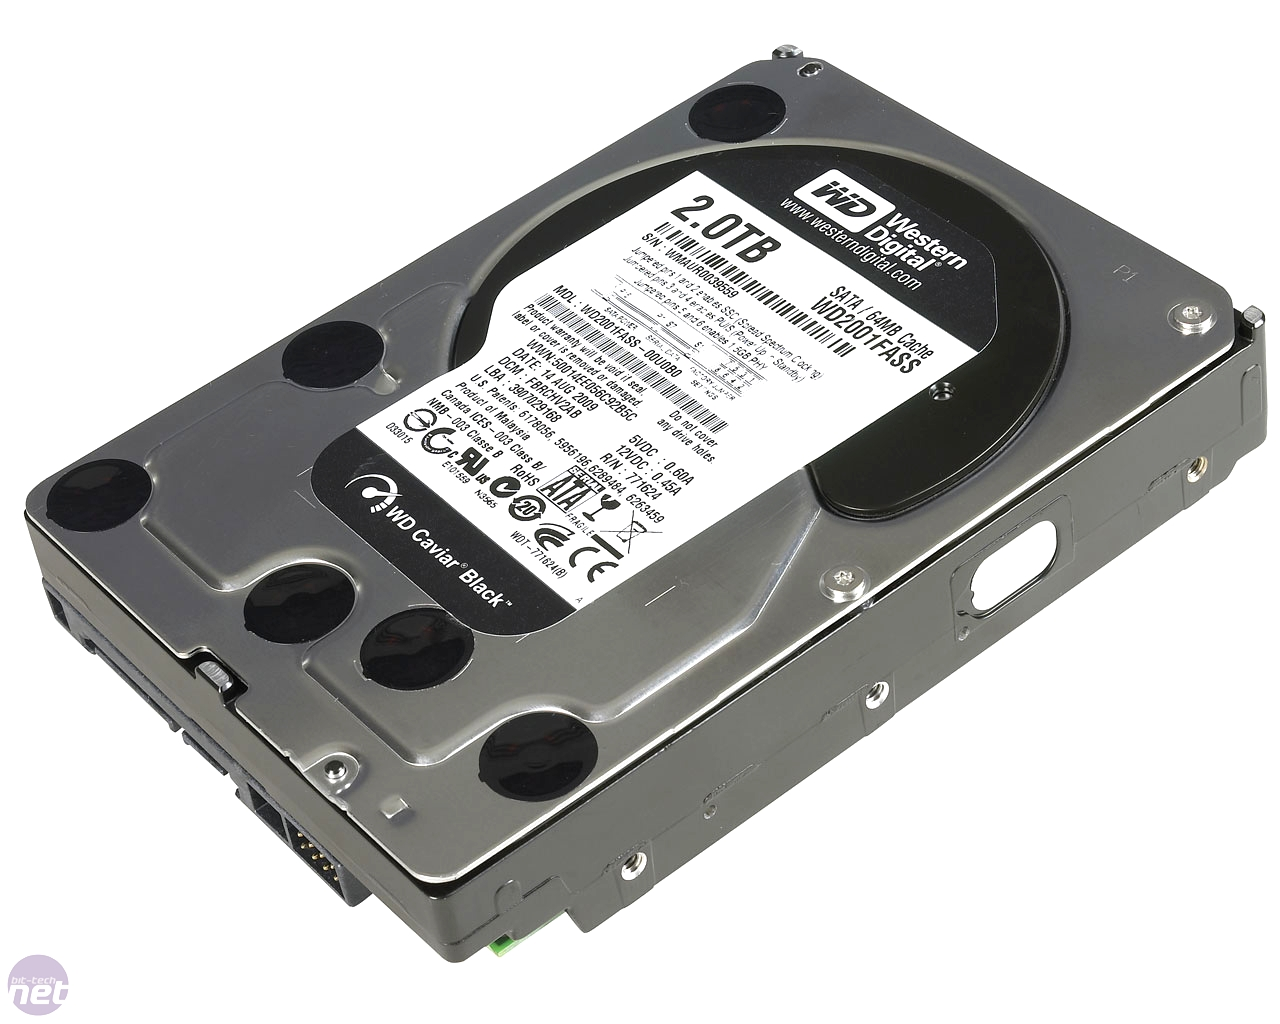
\includegraphics[width=0.9\linewidth]{figures/outsidedd.jpg}
    %\end{column}
    %\begin{column}{0.5\linewidth}
      %\centering
      %SSD

      %\medskip

      %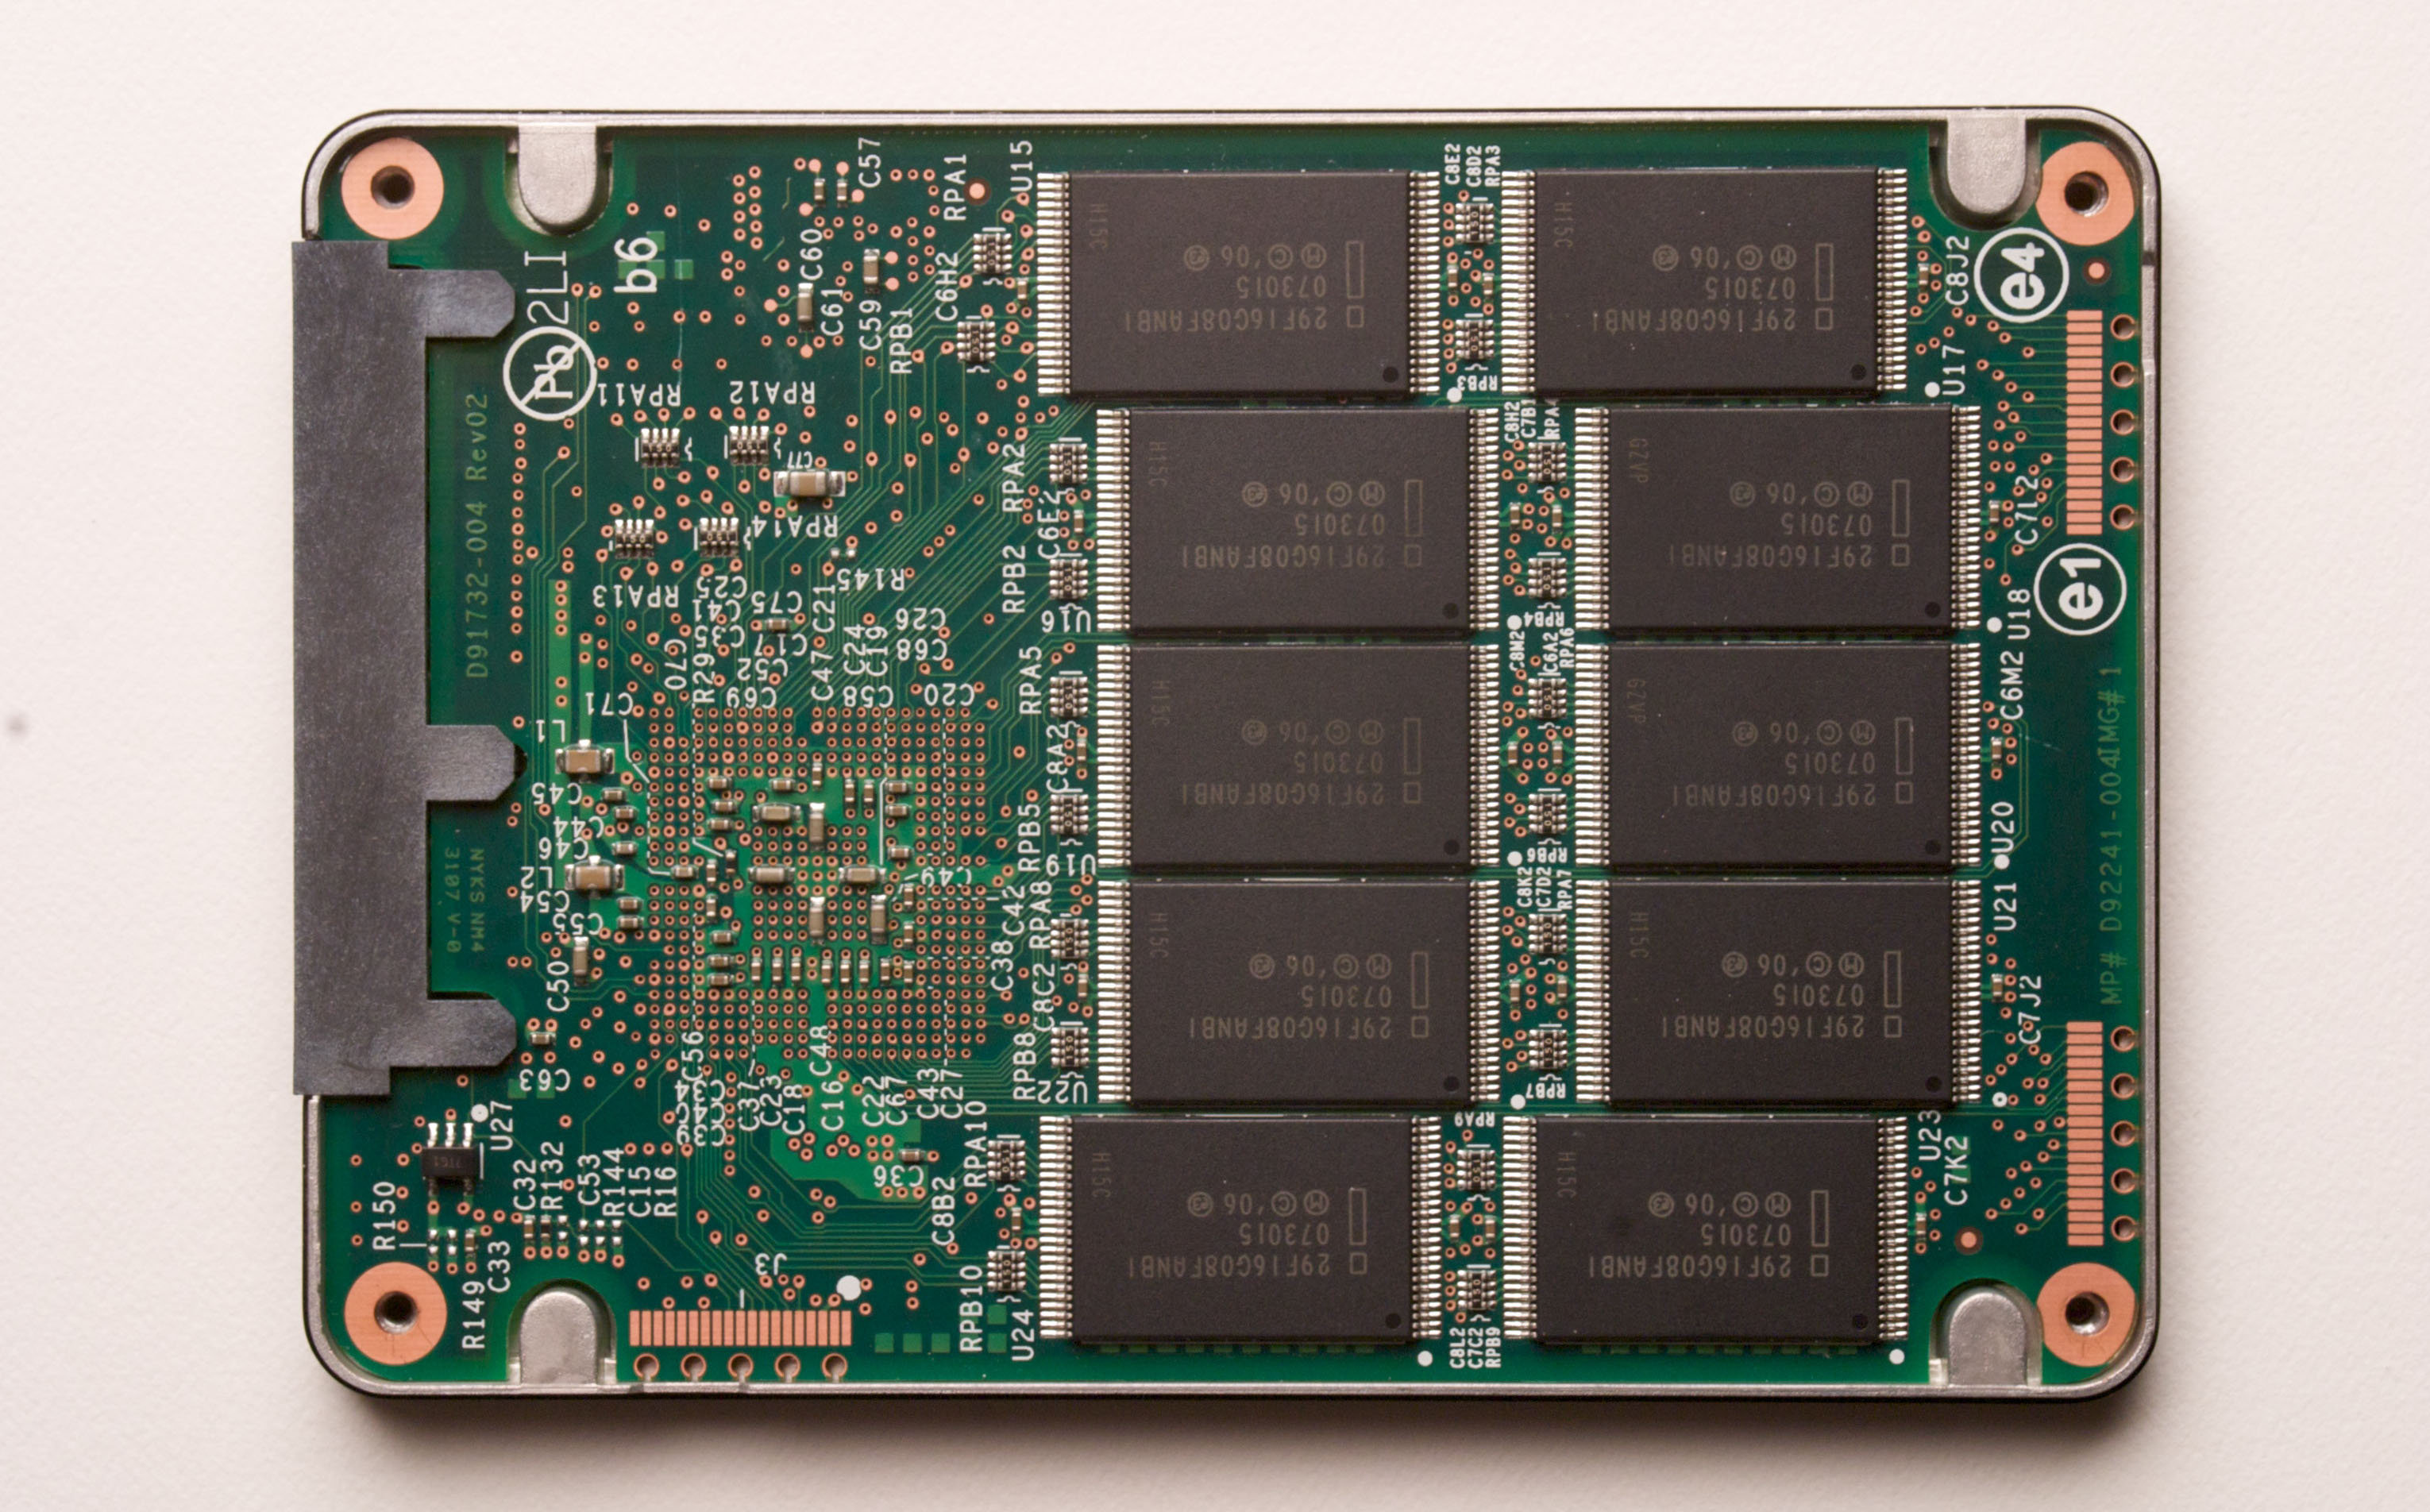
\includegraphics[width=0.9\linewidth]{figures/ssd.jpg}
    %\end{column}
  %\end{columns}
%}


%\frame{
  %\frametitle{Principe de fonctionnement d'un disque dur}

  %Stockage de masse persistant par modification du champ magnétique d'un matériau ferromagnétique

  %\bigskip

  %\begin{columns}
    %\begin{column}{0.5\linewidth}
      %\centering
      %\resizebox{0.95\linewidth}{!}{%% \documentclass{report}
%% \usepackage{fullpage}
%% \usepackage{tikz}
%% \usepackage[utf8]{inputenc}
%% \usepackage[OT1]{fontenc}

%% \begin{document}

\begin{tikzpicture}


\node at (5,-4) {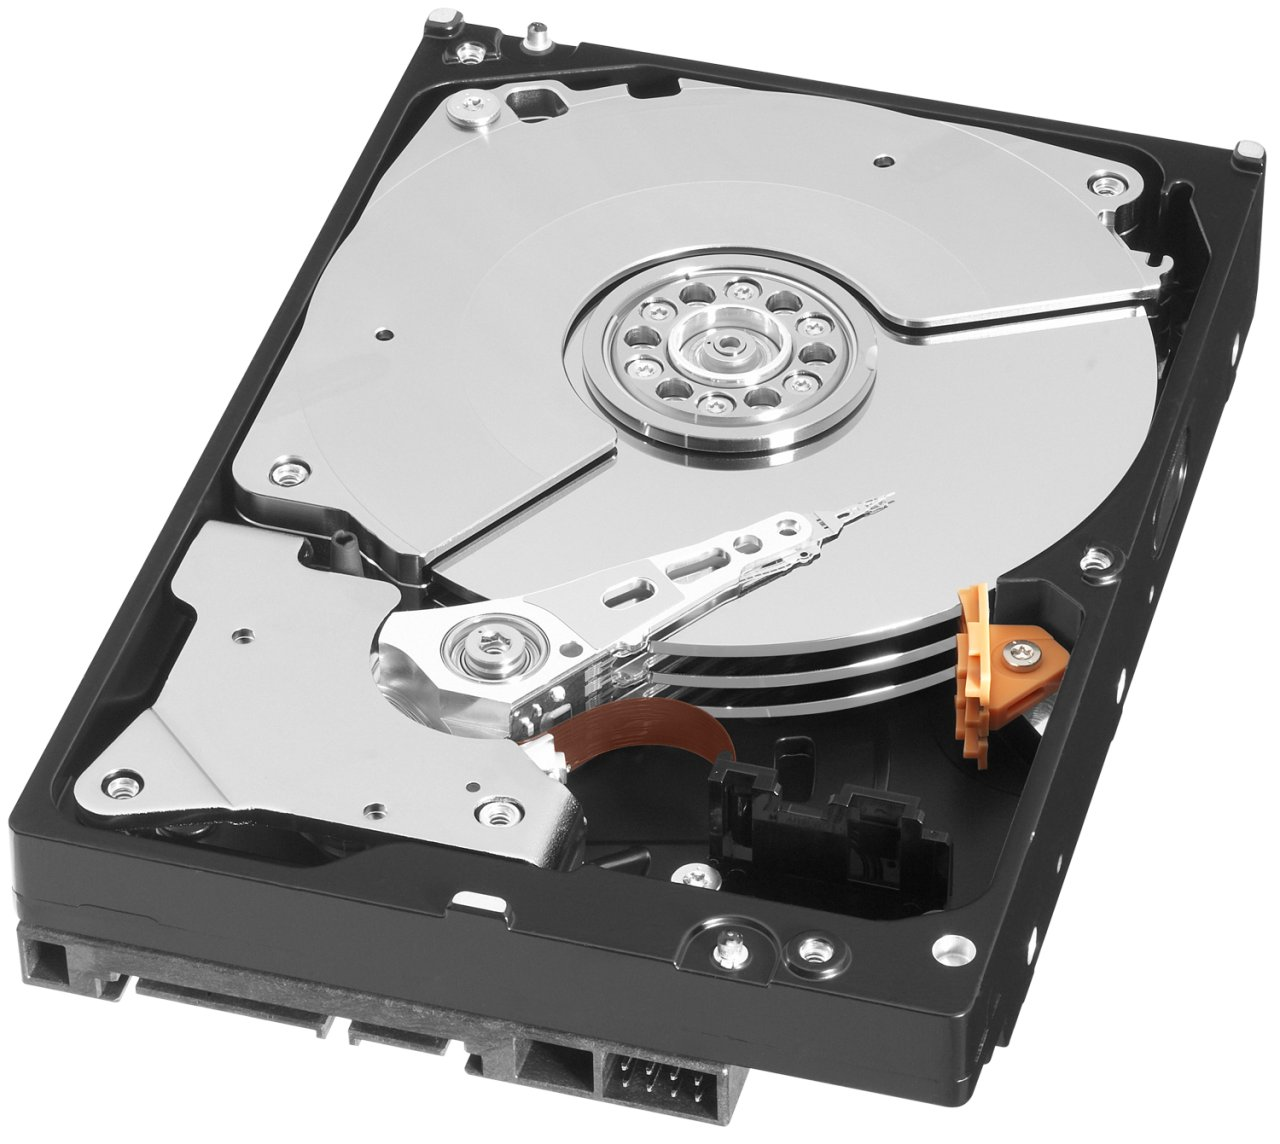
\includegraphics[width=8cm]{figures/insidedd.jpg}};


%% \foreach \i in {0,...,15} {
%%   \foreach \j in {-20,...,0} {
%%     \node[red] at (\i,\j) {\i,\j};
%%   }
%% }

\draw[blue,very thick] (7.5,-3) -- (8,-0.5) -- (9,-0.5);
\node[anchor=west] at (9,-0.5) {\Large Plateaux};

\draw[blue,very thick] (5.5,-2.6) -- (3,-0.5) -- (1.75,-0.5);
\node[anchor=east] at (1.75,-0.5) {\Large Axe de rotation};

\draw[blue,very thick] (6.5,-3.6) -- (8,-5) -- (9,-5);
\node[anchor=west] at (9,-5) {\Large Tête de lecture};

\draw[blue,very thick] (5.1,-7.2) -- (6,-8) -- (7.5,-8);
\node[anchor=west] at (7.5,-8) {\Large Alimentation};

\draw[blue,very thick] (5,-4.1) -- (3,-3) -- (1,-3);
\node[anchor=east] at (1,-3) {\Large Bras de lecture};

\draw[blue,very thick] (2.5,-6.6) -- (2,-7.5) -- (1,-7.5);
\node[anchor=east] at (1,-7.5) {\Large Interface};

\end{tikzpicture}

%\end{document}
}
    %\end{column}
    %\begin{column}{0.5\linewidth}
      %\centering
      %\resizebox{0.95\linewidth}{!}{%% \documentclass{report}
%% \usepackage{fullpage}
%% \usepackage{tikz}
%% \usepackage[utf8]{inputenc}
%% \usepackage[OT1]{fontenc}

%% \begin{document}

\begin{tikzpicture}


\draw[thick] (0,-2.4) -- (0,-4);

\draw[very thick,fill=white] (0,-2.4) ellipse (3cm and 1cm);
\draw[black!40,fill=blue!25] (0,-2.3) ellipse (2.7cm and 0.8cm);
\draw[black!40,fill=white] (0,-2.2) ellipse (2.3cm and 0.6cm);
\draw[black!40] (0,-2.1) ellipse (1.8cm and 0.4cm);
\draw[black!40] (0,-2) ellipse (1.3cm and 0.2cm);

\draw[very thick,fill=white] (0,-1.2) ellipse (3cm and 1cm);
\draw[black!40,fill=blue!25] (0,-1.1) ellipse (2.7cm and 0.8cm);
\draw[black!40,fill=white] (0,-1) ellipse (2.3cm and 0.6cm);
\draw[black!40] (0,-0.9) ellipse (1.8cm and 0.4cm);
\draw[black!40] (0,-0.8) ellipse (1.3cm and 0.2cm);

\draw[very thick,fill=white] (0,0) ellipse (3cm and 1cm);
\draw[black!40,fill=blue!25] (0,0.1) ellipse (2.7cm and 0.8cm);
\draw[black!40,fill=white] (0,0.2) ellipse (2.3cm and 0.6cm);
\draw[black!40] (0,0.3) ellipse (1.8cm and 0.4cm);
\draw[black!40] (0,0.4) ellipse (1.3cm and 0.2cm);
\draw[red!35,fill=red!35] (0,0.4) -- (1.2,-0.87) -- (2,-0.71) -- (0,0.4);
\draw[very thick] (0,0) ellipse (3cm and 1cm);
\draw[black!40] (0,0.1) ellipse (2.7cm and 0.8cm);
\draw[black!40] (0,0.2) ellipse (2.3cm and 0.6cm);
\draw[black!40] (0,0.3) ellipse (1.8cm and 0.4cm);
\draw[black!40] (0,0.4) ellipse (1.3cm and 0.2cm);

\draw[thick] (0,1.5) -- (0,0.4);


%% \foreach \i in {0,...,15} {
%%   \foreach \j in {-20,...,0} {
%%     \node[red] at (\i,\j) {\i,\j};
%%   }
%% }


\end{tikzpicture}

%\end{document}
}
    %\end{column}
  %\end{columns}
%}

%\frame{
  %\frametitle{Avantages et inconvénients d'un disque dur}

  %\begin{alertblock}{Avantages}
    %\begin{itemize}
      %\item Grande capacité (plusieurs TB)
      %\item Prix par octet
      %\item Durabilité du stockage magnétique
    %\end{itemize}
  %\end{alertblock}

  %\begin{alertblock}{Inconvénients}
    %\begin{itemize}
      %\item Lent (débit, et surtout \alert{latence})
      %\item Temps d'accès non homogène (la position des données sur le disque est importante)
      %\item Fragilité du système électro-mécanique
    %\end{itemize}
  %\end{alertblock}
%}

%\frame{
  %\frametitle{SSD : principe de fonctionnement}

  %SSD est l'acronyme de \textit{Solid State Drive}).

  %C'est un stockage de masse persistant en mémoire Flash

  %\bigskip

  %\begin{columns}
    %\begin{column}{0.5\textwidth}
      %Une cellule de mémoire Flash est construite autour d'un transistor à grille flottante qui permet \textit{d'emprisonner} des électrons et ainsi stocker 1 bit.

    %\end{column}
    %\begin{column}{0.5\linewidth}
      %\centering
      %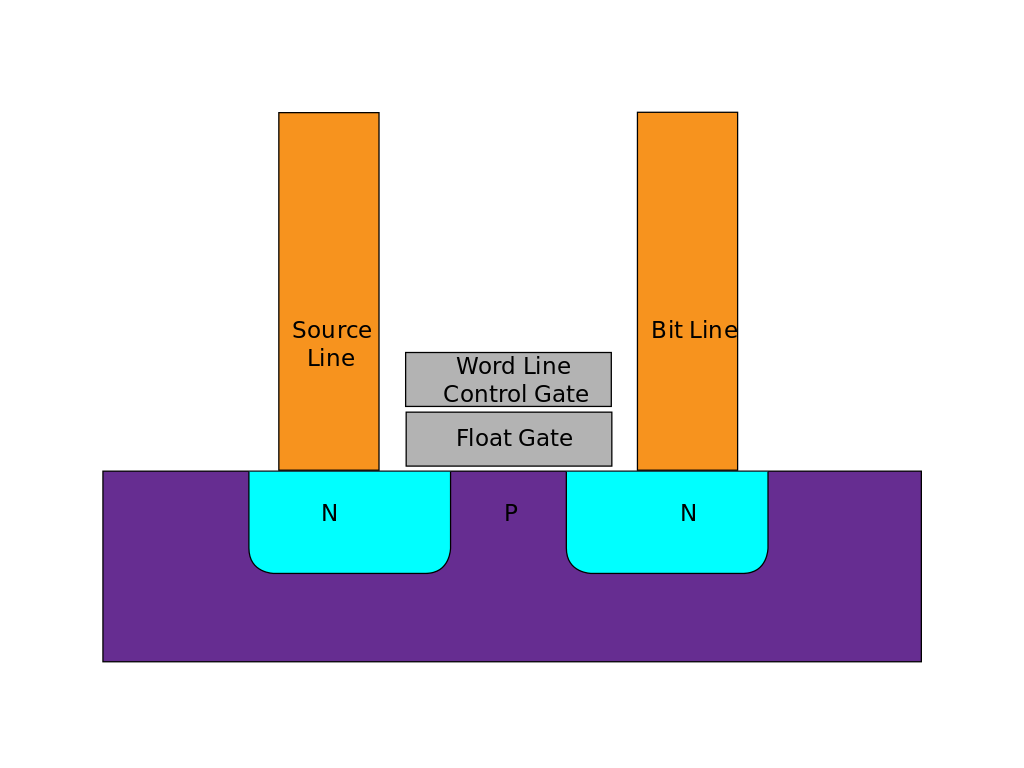
\includegraphics[width=0.9\linewidth]{figures/Flash_cell}
    %\end{column}
  %\end{columns}
%}

%\frame{
  %\frametitle{Avantages et inconvénients d'un disque SSD}
  %\begin{alertblock}{Avantages}
    %\begin{itemize}
      %\item Rapidité (latence et débit)
      %\item Robustesse (absence de pièce mécanique)
    %\end{itemize}
  %\end{alertblock}

  %\begin{alertblock}{Inconvénients}
    %\begin{itemize}
      %\item Prix par octet
      %\item Importance du \textit{firmware} et du pilote sur les performances et la durée de vie
      %\item Peu adapté aux systèmes réalisant des écritures répétées (capture vidéo)
      %\item Durabilité réduite de la technologie de stockage (environ 10 ans avec les techno. actuelles)
    %\end{itemize}
  %\end{alertblock}
%}

%\frame{
  %\frametitle{Transport de l'information : les bus}

  %\begin{columns}
    %\begin{column}{0.6\linewidth}
      %\alert{Bus} = ensemble de fils électriques.

      %\medskip

      %Les bus sont conçus pour transmettre des \alert{mots} de taille fixe (de 8 à 64 bits), qui peuvent être une/des commande(s), une adresse, ou une/des donnée(s).
    %\end{column}
    %\begin{column}{0.4\linewidth}
      %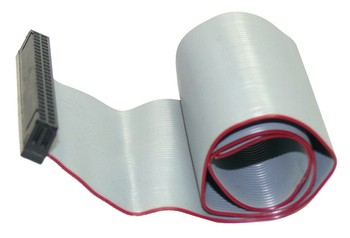
\includegraphics[width=4cm]{figures/bus.JPG}
    %\end{column}
  %\end{columns}

  %\bigskip

  %\begin{columns}[t]
    %\begin{column}{0.5\linewidth}
      %\alert{Bus parallèle} : $n$ fils ($n$ = largeur du mot), mots transmis un bit par fil.

      %\medskip

      %Exemple : processeur ↔ mémoire (données, adresse, contrôle, horloge)
    %\end{column}
    %\begin{column}{.5\linewidth}
      %\alert{Bus série} : 1 fil, mot transmis bit après bit

      %\medskip

      %Exemple : disque dur SATA (Serial ATA).
    %\end{column}
  %\end{columns}

%}

%% ajouter un exemple d'écriture dans la ram ?

%\frame{
  %\frametitle{La mémoire centrale (non persistante)}

  %\begin{block}{Principalement : DRAM}
    %Dynamic Random Access Memory
  %\end{block}

  %\begin{center}
    %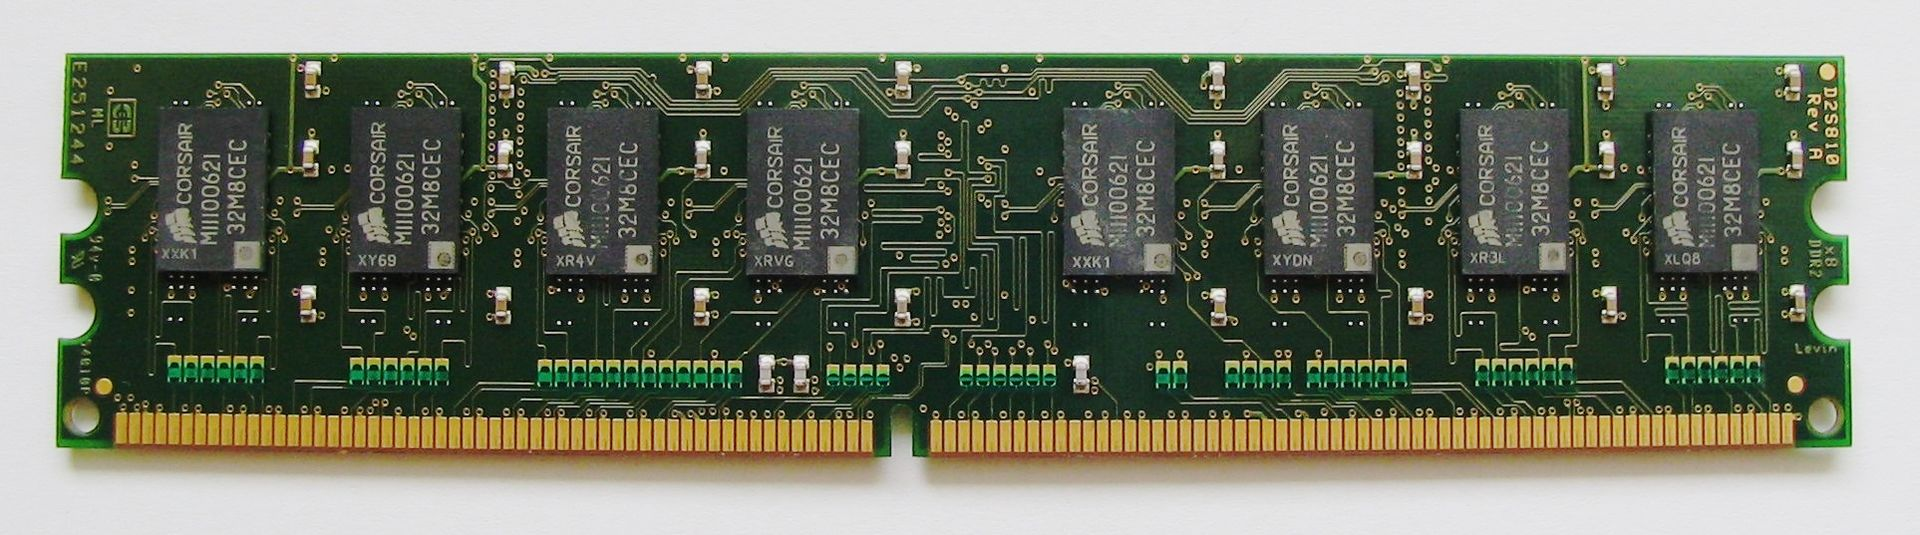
\includegraphics[width=10cm]{figures/dram.jpg}
  %\end{center}

  %\begin{block}{Caractéristiques}
    %\begin{itemize}
      %\item Stockage d'un bit : charge d'un condensateur $\rightarrow$ nécessité de rafraîchir la mémoire (chaque 10 à 100 ms)
      %\item Données stockées dans des supercellules (généralement \SI{8}{\bit}) organisées en grille
      %\item Logique d'accès réalisée à l'aide de transistors CMOS
    %\end{itemize}
  %\end{block}


%}


%\section{Quelques mots sur la hiérarchie de la mémoire}

%\frame{
  %\frametitle{Hiérarchie de la mémoire, principe}

  %\scalebox{0.7}{%% \documentclass{report}
%% \usepackage{fullpage}
%% \usepackage{tikz}
%% \usepackage[utf8]{inputenc}
%% \usepackage[OT1]{fontenc}

%% \begin{document}

\begin{tikzpicture}

%registres
\draw (8,0) -- (7,-2) -- (9,-2) -- (8,0);
\node at (8,-1.35) {\Large Reg.};

%cache L1
\draw (7,-2) -- (6.5,-3) -- (9.5,-3) -- (9,-2);
\node at (8,-2.5) {\Large Cache L1};

%cache L2
\draw (6.5,-3) -- (6,-4) -- (10,-4) -- (9.5,-3);
\node at (8,-3.5) {\Large Cache L2};

% cache L3
\draw (6,-4) -- (5, -6) -- (11,-6) -- (10,-4);
\node at (8, -5) {\Large Cache L3};

%mémoire
\draw (5,-6) -- (4,-8) -- (12,-8) -- (11,-6);
\node at (8,-7) {\Large Mémoire};

%disque
\draw (4,-8) -- (3,-10) -- (13,-10) -- (12,-8);
\node at (8,-9) {\Large Stockage de masse};


\newcommand{\myarrowup}[4]{% x depart, y depart, longueur
\draw[#4,fill=#4] (#1+0.25,#2) -- (#1+0.25,#2+#3-0.5) -- (#1+0.5,#2+#3-0.5) -- (#1,#2+#3) -- (#1-0.5,#2+#3-0.5) -- (#1-0.25,#2+#3-0.5) -- (#1-0.25,#2) -- (#1+0.25,#2);
}
\newcommand{\myarrowdown}[4]{% x depart, y depart, longueur
\draw[#4,fill=#4] (#1+0.25,#2) -- (#1+0.25,#2-#3+0.5) -- (#1+0.5,#2-#3+0.5) -- (#1,#2-#3) -- (#1-0.5,#2-#3+0.5) -- (#1-0.25,#2-#3+0.5) -- (#1-0.25,#2) -- (#1+0.25,#2);
}

\myarrowdown{0}{0}{10}{white}


\only<4->{
%cout
\myarrowup{1}{-10}{10}{red!50}
\node[rotate=90] at (1,-5) {\Large Prix du bit};
\node at (1,-9.5) {\Huge -};
\node at (1,-0.5) {\Large +};
}

\only<3->{
%taille
\myarrowdown{0}{0}{10}{blue!25}
\node[rotate=90] at (0,-5) {\Large Taille};
\node at (0,-9.5) {\Large +};
\node at (0,-0.5) {\Huge -};
}

\only<2->{
%rapidité
\myarrowup{2}{-10}{10}{teal!50}
\node[rotate=90] at (2,-5) {\Large Rapidité de l'accès aux données};
\node at (2,-9.5) {\Huge -};
\node at (2,-0.5) {\Large +};
}



%% \foreach \i in {0,...,15} {
%%   \foreach \j in {-20,...,0} {
%%     \node[black!25] at (\i,\j) {\i,\j};
%%   }
%% }

\end{tikzpicture}

%\end{document}
}

%}

%\frame{
  %\frametitle{Principe de fonctionnement de la hiérarchie mémoire}

  %Chaque niveau sert de \alert{cache} au niveau suivant :
  %\begin{itemize}
    %\item contient un petit sous-ensemble des données du niveau suivant
    %\item offre un accès plus rapide à ces données
  %\end{itemize}

  %\medskip

  %L'accès se fait toujours au niveau le plus haut.
  %Si la donnée recherchée n'est pas présente, elle est chargée depuis les niveaux inférieurs vers les niveaux supérieurs puis l'accès est recommencé.
  %\alert{Les transferts se font uniquement entre niveaux voisins}.

  %\medskip

  %Attention :
  %\begin{itemize}
    %\item Quand une donnée est modifiée, il faut propager vers les niveaux inférieurs
    %\item Dans les systèmes multiprocesseurs, plusieurs niveaux sont présents en plusieurs exemplaires (L1, L2) : il faut assurer leur cohérence.
  %\end{itemize}
%}

%\frame{
  %\frametitle{Localités spatiale et temporelle}

  %Pour que la hiérarchie mémoire fonctionne bien, il faut que les données cachées (= les données des niveaux supérieurs) soient bien choisies.

  %\medskip

  %\begin{alertblock}{Localité spatiale}
    %Si une donnée est utilisée, les données proches (c'est-à-dire situées à des adresses mémoire proches) seront sans doute bientôt utiles.
  %\end{alertblock}

  %\medskip

  %\begin{alertblock}{Localité temporelle}
    %Une donnée qui vient d'être utilisée sera sans doute bientôt utile à nouveau dans un avenir proche.
  %\end{alertblock}

%}

%\frame{
  %\frametitle{Pourquoi un système aussi compliqué ?}


  %\href{https://gist.github.com/jboner/2841832}{Latency numbers every programmer should know}

%}

%\section{Le processeur}

%\frame{
  %\frametitle{Deuxième étape : exécution depuis la mémoire}

  %Une fois le programme chargé, le processeur peut commencer à exécuter la liste des instructions qu'il contient.

  %\medskip

  %Les instructions sont lues depuis la mémoire puis décodées et exécutées dans le processeur.

  %\medskip

  %En plus des calculs, le processeur lit et écrit en mémoire les données manipulées par le programme.

  %\medskip

  %Les instructions du programme peuvent également amener le processeur a accéder aux autres périphériques d'entrée-sortie de la machine.
%}
%\frame{
  %\centering
  %\scalebox{0.7}{%% \documentclass{report}
%% \usepackage{fullpage}
%% \usepackage{tikz}
%% \usepackage[utf8]{inputenc}
%% \usepackage[OT1]{fontenc}

%% \begin{document}

\begin{tikzpicture}

\newcommand{\myarrowright}[3]{% x depart, y depart, longueur
\draw[black!25,fill=black!25] (#1,#2+0.25) -- (#1+#3-0.5,#2+0.25) -- (#1+#3-0.5,#2+0.5) -- (#1+#3,#2) -- (#1+#3-0.5,#2-0.5) -- (#1+#3-0.5,#2-0.25) -- (#1,#2-0.25) -- (#1,#2+0.25);
}
\newcommand{\myarrowleft}[3]{% x depart, y depart, longueur
\draw[black!25,fill=black!25] (#1,#2+0.25) -- (#1-#3+0.5,#2+0.25) -- (#1-#3+0.5,#2+0.5) -- (#1-#3,#2) -- (#1-#3+0.5,#2-0.5) -- (#1-#3+0.5,#2-0.25) -- (#1,#2-0.25) -- (#1,#2+0.25);
}
\newcommand{\myarrowup}[3]{% x depart, y depart, longueur
\draw[black!25,fill=black!25] (#1+0.25,#2) -- (#1+0.25,#2+#3-0.5) -- (#1+0.5,#2+#3-0.5) -- (#1,#2+#3) -- (#1-0.5,#2+#3-0.5) -- (#1-0.25,#2+#3-0.5) -- (#1-0.25,#2) -- (#1+0.25,#2);
}
\newcommand{\myarrowdown}[3]{% x depart, y depart, longueur
\draw[black!25,fill=black!25] (#1+0.25,#2) -- (#1+0.25,#2-#3+0.5) -- (#1+0.5,#2-#3+0.5) -- (#1,#2-#3) -- (#1-0.5,#2-#3+0.5) -- (#1-0.25,#2-#3+0.5) -- (#1-0.25,#2) -- (#1+0.25,#2);
}


%% \foreach \i in {0,...,15} {
%%   \foreach \j in {-20,...,0} {
%%     \node[black!25] at (\i,\j) {\i,\j};
%%   }
%% }

%cpu
\draw (0,0) rectangle (7,-6);
\node at (8.25,-0.25) {\Large Processeur};
%bus registers->ALU
\myarrowright{3.75}{-1.5}{1.25}
%bus ALU->registers
\myarrowleft{5}{-3}{1.25}
%bus CPU->i/o bridge
\myarrowright{6}{-5.25}{2}
%bus i/o bridge->CPU
\myarrowleft{7}{-5.25}{2}
%bus i/o brige->memory
\myarrowright{11}{-5.25}{2.5}
%bus memory->i/o bridge
\myarrowleft{11}{-5.25}{1}
%i/o bus->i/o bridge
\myarrowup{9}{-7}{1.25}
%bus interface->registers
\myarrowup{3}{-4}{0.5}
%registers->bus interface
\myarrowdown{3}{-4}{0.75}
%i/o bus->usb controller
\myarrowdown{2}{-7.25}{1.5}
%i/o bus->graphics adapter
\myarrowdown{6}{-7.25}{1.5}
%i/o bus->disk controller
\myarrowdown{10}{-7.25}{1.5}
%pc
\draw (0.5,-1.75) rectangle (2,-2.25);
\node at (1.25,-2) {\Large PC};
%other registers
\draw (2.25,-1) rectangle (3.75,-3.5);
\draw (2.25,-1.5) -- (3.75,-1.5);
\draw (2.25,-2) -- (3.75,-2);
\draw (2.25,-2.5) -- (3.75,-2.5);
\draw (2.25,-3) -- (3.75,-3);
\node at (2,-0.5) {\Large Registres};
%alu
\draw (5,-0.5) rectangle (6.5,-4);
\node at (5.75,-2.25) {\Large UAL};
%bus interface
\draw (0.5,-4.75) rectangle (5,-5.75);
\node at (2.75,-5.25) {\Large Interface};
%i/o bridge
\draw (8,-4.75) rectangle (10,-5.75);
\node at (9,-5.25) {\large Pont e/s};
%memory
\draw (13.5,-4) rectangle (15.5,-6);
\node at (14.5,-5) {\Large Mémoire};
%i/o bus
\myarrowleft{8}{-7.25}{8}
\myarrowright{8}{-7.25}{7.5}
%usb controller
\draw (1,-8.75) rectangle (3,-9.75);
\node at (2,-9) {\large Contrôleur};
\node at (2,-9.5) {\large USB};
\draw[-latex] (1.25,-10.5) -- (1.25,-9.75);
\node at (1.25,-10.75) {\Large Clavier~~~};
\draw[-latex] (2.75,-10.5) -- (2.75,-9.75);
\node at (2.75,-10.75) {\Large ~~~Souris};
%graphics adapter
\draw (4.95,-8.75) rectangle (7.05,-9.75);
\node at (6,-9) {\large Adaptateur};
\node at (6,-9.5) {\large graphique};
\draw[-latex] (6,-9.75) -- (6,-10.5);
\node at (6,-10.75) {\Large Écran};
%disk controller
\draw (9,-8.75) rectangle (11,-9.75);
\node at (10,-9) {\large Contrôleur};
\node at (10,-9.5) {\large Stockage};
\draw[-latex] (11,-9.25) -- (12.5,-9.25);
\draw[-latex] (12.5,-9.25) -- (11,-9.25);
%disk
\draw (12.5,-8.5) rectangle (14.5,-10.5);
\node at (13.5,-9.5) {\Large Disque};
%bus names
\node at (7.5,-7.25) {\large Bus e/s};
\node at (11.75,-5.25) {\large Bus mémoire};
\node at (6.5,-5.25) {\large Bus système};


\draw[red,very thick] (3,-3) -- (5.75,-3) -- (5.75,-1.5) -- (3,-1.5) -- (3,-5.25) -- (13.6,-5.25);
\node[red] at (14.5,-5.5) {\large \tt hello};

\end{tikzpicture}

%\end{document}
}
%}

%\frame{
  %\frametitle{Le processeur}

  %Il est cadencé par une horloge interne construite autour d'un crystal de quartz : à chaque top il exécute une (partie d'une) \alert{instruction}.

  %C'est le \alert{compteur de programme} qui indique l'adresse en mémoire de l'instruction suivante.

  %\medskip

  %\begin{columns}[c]
    %\begin{column}{6cm}
      %\centering
      %\scalebox{0.6}{%% \documentclass{report}
%% \usepackage{fullpage}
%% \usepackage{tikz}
%% \usepackage[utf8]{inputenc}
%% \usepackage[OT1]{fontenc}

%% \begin{document}

\begin{tikzpicture}

\newcommand{\myarrowright}[3]{% x depart, y depart, longueur
\draw[black!25,fill=black!25] (#1,#2+0.25) -- (#1+#3-0.5,#2+0.25) -- (#1+#3-0.5,#2+0.5) -- (#1+#3,#2) -- (#1+#3-0.5,#2-0.5) -- (#1+#3-0.5,#2-0.25) -- (#1,#2-0.25) -- (#1,#2+0.25);
}
\newcommand{\myarrowleft}[3]{% x depart, y depart, longueur
\draw[black!25,fill=black!25] (#1,#2+0.25) -- (#1-#3+0.5,#2+0.25) -- (#1-#3+0.5,#2+0.5) -- (#1-#3,#2) -- (#1-#3+0.5,#2-0.5) -- (#1-#3+0.5,#2-0.25) -- (#1,#2-0.25) -- (#1,#2+0.25);
}
\newcommand{\myarrowup}[3]{% x depart, y depart, longueur
\draw[black!25,fill=black!25] (#1+0.25,#2) -- (#1+0.25,#2+#3-0.5) -- (#1+0.5,#2+#3-0.5) -- (#1,#2+#3) -- (#1-0.5,#2+#3-0.5) -- (#1-0.25,#2+#3-0.5) -- (#1-0.25,#2) -- (#1+0.25,#2);
}
\newcommand{\myarrowdown}[3]{% x depart, y depart, longueur
\draw[black!25,fill=black!25] (#1+0.25,#2) -- (#1+0.25,#2-#3+0.5) -- (#1+0.5,#2-#3+0.5) -- (#1,#2-#3) -- (#1-0.5,#2-#3+0.5) -- (#1-0.25,#2-#3+0.5) -- (#1-0.25,#2) -- (#1+0.25,#2);
}


%% \foreach \i in {0,...,15} {
%%   \foreach \j in {-20,...,0} {
%%     \node[black!25] at (\i,\j) {\i,\j};
%%   }
%% }

%cpu
\draw (0,0) rectangle (7,-6);
%\node at (8.25,-0.25) {\Large Processeur};
%bus registers->ALU
\myarrowright{3.75}{-1.5}{1.25}
%bus ALU->registers
\myarrowleft{5}{-3}{1.25}
%bus interface->registers
\myarrowup{3}{-4}{0.5}
%registers->bus interface
\myarrowdown{3}{-4}{0.75}
%pc
\draw (0.5,-1.75) rectangle (2,-2.25);
\node at (1.25,-2) {\Large PC};
%other registers
\draw (2.25,-1) rectangle (3.75,-3.5);
\draw (2.25,-1.5) -- (3.75,-1.5);
\draw (2.25,-2) -- (3.75,-2);
\draw (2.25,-2.5) -- (3.75,-2.5);
\draw (2.25,-3) -- (3.75,-3);
\node at (2,-0.5) {\Large Registres};
%alu
\draw (5,-0.5) rectangle (6.5,-4);
\node at (5.75,-2.25) {\Large UAL};
%bus interface
\draw (0.5,-4.75) rectangle (5,-5.75);
\node at (2.75,-5.25) {\Large Interface};

\end{tikzpicture}

%\end{document}
}
    %\end{column}
    %\begin{column}{5.5cm}
      %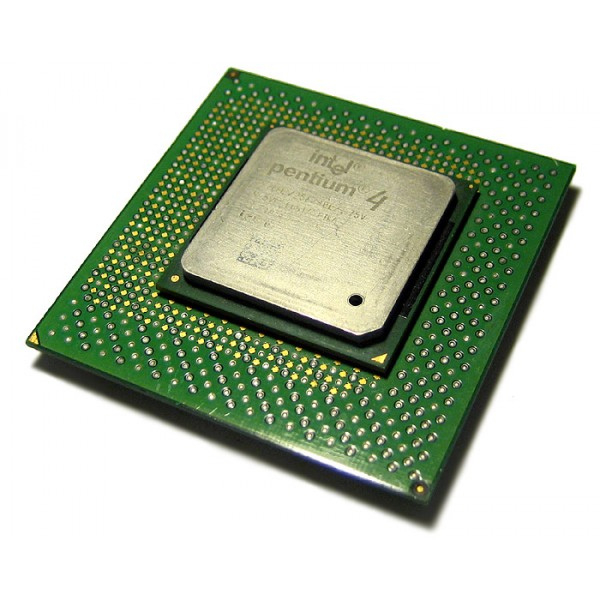
\includegraphics[width=5cm]{figures/proc.jpg}
    %\end{column}
  %\end{columns}

%}

%\frame{
  %\frametitle{Les registres}

  %Le processeur contient de la mémoire : des \alert{registres} de tailles fixes (1 mot mémoire).
  %Pour assurer des accès ultra-rapides, ils sont conçus en SRAM (Static RAM, stockage via des transistors CMOS)

  %\medskip

  %Certains sont visibles du programme, qui y accède par leur \alert{nom}.
  %La plupart servent à stocker les opérandes et/ou les résultats des instructions exécutées par le processeur.

  %D'autres ont un rôle particulier, par exemple :
  %\begin{itemize}
    %\item le compteur de programme,
    %\item le registre de status,
    %\item ou encore le pointeur de pile,
  %\end{itemize}

  %\medskip

  %Le processeur contient également des registres privés, utiles pour son fonctionnement interne.

%}

%\frame{
  %\frametitle{Unité arithmétique et logique}

  %Au sein d'un processeur, une \alert{unité arithmétique et logique} (UAL, ou \textit{ALU}) est un organe chargé de réaliser les calculs.
  %Les processeurs modernes disposent de plusieurs UALs.

  %Les UALs élémentaires fournissent des opérations d'arithmétique entière et de logique (cf. TP).

  %\medskip

  %D'autres UALs sont spécialisées pour l'arithmétique des nombres à virgule flottante (\textit{FPU}).

  %\medskip

  %Enfin, des UALs spécialisées ont été développées pour accélérer certains calculs (p. ex. les unités vectorielles)
%}

%\section{Le langage machine}

%\frame{
  %\frametitle{Le langage machine}

  %Pour exécuter \texttt{hello}, le processeur exécute une séquence d'instructions.

  %Une instruction = une opération + des opérandes.

  %La séquence est codée en binaire dans la section \texttt{.text} du fichier ELF contenant le programme, qui a été copiée en mémoire lors de l'étape précédente.

  %Ce qu'on appelle \alert{langage machine} c'est à la fois :
  %\begin{itemize}
    %\item la liste des opérations et les opérandes qu'elles supportent,
    %\item et la façon de les coder en binaire.
  %\end{itemize}

  %Il existe une syntaxe textuelle qu'on appelle assembleur (ou langage d'assemblage).

%}


%\frame{
  %\frametitle{Quelques opérations que peut réaliser un processeur}

  %\begin{block}{Load}
    %Écriture d'un mot de la mémoire vers un registre.
  %\end{block}

  %\begin{block}{Store}
    %Écrire d'un mot d'un registre vers la mémoire.
  %\end{block}

  %\begin{block}{Add, Sub, And, Shift, \ldots}
    %Faire une opération arithmétique ou logique dont la ou les opérandes (sources et cibles) sont des registres.
  %\end{block}

  %\begin{block}{Branch (ou jump)}
    %Sauter vers une instruction donnée, éventuellement sous certaines conditions.
  %\end{block}
%}


%\frame{
  %\frametitle{Jeu d'instruction CISC vs. RISC}

  %\begin{remarque}{ISA vs. microarchitecture}
    %La traduction en anglais de jeu d'instruction est \textit{instruction set architecture}.

    %L'ISA est l'interface de programmation de la machine proposée aux utilisatrices et utilisateurs.

    %L'implémentation de l'ISA sous forme de circuits est appelée la microarchitecture du processeur.
  %\end{remarque}


  %\begin{block}{ISA CISC : \textit{Complex Instruction Set Computers}}
    %\begin{itemize}
      %\item Beaucoup d'instructions
      %\item Des instructions complexes/longues à exécuter
    %\end{itemize}
  %\end{block}

  %\medskip

  %\begin{block}{ISA RISC : \textit{Reduced Instruction Set Computers}}
    %\begin{itemize}
      %\item Nombre (volontairement) limité d'instructions (<100 à l'origine)
      %\item Des instructions basiques/rapides à exécuter
    %\end{itemize}
  %\end{block}

  %\medskip

  %Beaucoyp de processeurs combinent les deux approches :
  %\begin{itemize}
    %\item Intel/AMD : ISA CISC implémenté par microcodage sur une microarchitecture RISC
    %\item ARM : ISA RISC à l'origine qui intègre des instructions complexes au fur et à mesure des évolutions
  %\end{itemize}
%}

%\section{Exécution des instructions}


%\begin{frame}
  %\frametitle{Exécution d'une instruction}

  %On décompose classiquement l'exécution d'une instruction en plusieurs étapes :
  %\begin{enumerate}
    %\item \alert{Fetch} : l'instruction est lue depuis la mémoire
    %\item \alert{Decode} : l'instruction est décodée
    %\item \alert{Execute} : exécute l'instruction (par exemple en utilisant l'UAL)
    %\item  \alert{Mem} : si l'instruction est un accès mémoire, un second cycle est nécessaire
    %\item \alert{Writeback} : le résultat de l'instruction est écrit dans les registres cibles
  %\end{enumerate}
%\end{frame}

%\begin{frame}
  %\frametitle{Pipeline, superscalaire, exécution dans le désordre}
  %Les processeurs modernes utilisent un \alert{pipeline} à plusieurs étages :

  %\begin{itemize}
    %\item chaque étage correspond à une étape de l'exécution d'une instruction., plusieurs instructions sont donc simultanément dans le pipeline.
    %\item un processeur peut utiliser plusieurs pipeline en parallèle : on parle de processeur \alert{superscalaire}.
    %\item pour exploiter au mieux le pipeline, les processeurs peuvent exécuter les instructions \og \alert{dans le désordre} \fg (\textit{Out-of-Order}). Pour cela, ils détectent les dépendances entre les instructions.
    %\item pour ne pas être bloqué à attendre un résultat, les processeurs hautes performances intègrent des mécanismes d'\alert{exécution spéculative}.
  %\end{itemize}
%\end{frame}

%\section{En pratique}

%\begin{frame}[fragile]
  %\frametitle{Source → Exécutable}

  %On construit un fichier exécutable à partir du fichier source. Cela se fait avec une commande

  %\begin{tcolorbox}
    %\verb|go build|
  %\end{tcolorbox}

  %qui enchaîne plusieurs étapes :
  %\begin{itemize}
    %\item analyse lexicale
    %\item pré-processing
    %\item analyse syntaxique
    %\item analyse sémantique
    %\item génération de code et optimisations (→ code objet)
    %\item édition des liens
    %\item assemblage (→ exécutable)
  %\end{itemize}

%\end{frame}

%\begin{frame}[fragile]
  %\frametitle{Source → Code objet}

  %On peut stopper la procédure à l'étape d'émission du code objet avec la commande suivante :

  %\begin{tcolorbox}
    %\verb|go tool compile main.go|
  %\end{tcolorbox}


  %\medskip

  %On peut demander au compilateur d'émettre le code assembleur :

  %\begin{tcolorbox}
    %\verb|go tool compile -S -S main.go|
  %\end{tcolorbox}

  %ou

  %\begin{tcolorbox}
    %\verb|go build -gcflags '-S -S'|
  %\end{tcolorbox}

%\end{frame}

%\begin{frame}[fragile]
  %\frametitle{Code objet → code binaire}

  %\begin{remarque}
    %La chaîne de développement Go utilise est un assembleur « portable ».
    %Il est traduit vers l'assembleur de la machine cible lors de la phase d'édition des liens.
  %\end{remarque}

  %À partir du fichier objet, on peut obtenir le code exécutable en réalisation l'édition des liens :

  %\begin{tcolorbox}
    %\verb|go tool link main.o|
  %\end{tcolorbox}

  %Le code du \textit{runtime} Go et des fonctions externes est automatiquement ajouté dans l'exécutable.

  %Le fichier de sortie est un binaire au format ELF (Executable and Linkable Format)

%\end{frame}

%\begin{frame}[fragile]
  %\frametitle{Lancer l'exécution du programme}

  %Une fois le programme construit, on peut le lancer à l'aide de la commande :

  %\begin{tcolorbox}
    %\verb|./hello|
  %\end{tcolorbox}

  %qui enchaine plusieurs étapes :
  %\begin{itemize}
    %\item création d'un nouveau processus    \item initialisation de l'espace d'adressage du processus :
          %\begin{itemize}
            %\item chargement du programme dans la mémoire de travail
            %\item chargement des données initialisées dans la mémoire de travail
          %\end{itemize}
    %\item initialisation du pointeur d'instruction
    %\item exécution du programme instruction par instruction
  %\end{itemize}

%\end{frame}

%\begin{frame}{Observer l'exécution avec un debugger}

  %Un debugger est un outil qui permet d'exécuter un programme pas-à-pas et d'observer le contenu de sa mémoire.

  %On utilisera GDB (cf. tp n°1), un outil libre et gratuit, largement utilisé, qui permet d'observer l'exécution à deux niveaux :

  %\begin{itemize}
    %\item au niveau du langage source

    %\item au niveau ISA
  %\end{itemize}

  %\begin{remarque}
    %Pour observer l'exécution d'un programme au niveau de la microarchitecture, il faut passer par un émulateur ou un simulateur.
  %\end{remarque}

%\end{frame}

\end{document}
